\chapter{Bijou 7.1.0 Release Evidence}\label{record-260}

\noindent{\footnotesize\color{BookMuted}\path{docs/releases/7.1.0/README.md}\par}\smallskip

Bijou 7.1.0 is the post-V7 minor release that turns the accumulated V8-facing proof work into a clean public package boundary without expanding the release train. It ships the Runtime Graph and Scene IR seed work, the first GraphQL-authored DOGFOOD block fixture, theme/token polish, raster-to-glyph tooling, terminal-rendering fixes, and release-prep guardrails that make the next release checklist auditable.

This packet was prepared on the release branch before the public tag existed. The release tag and tag push are final-main steps and are excluded from this prep branch by operator instruction.

\section{Release Summary}\label{record-260-release-summary}

\begin{itemize}
\tightlist
\item
  Version: \texttt{7\allowbreak{}.\allowbreak{}1\allowbreak{}.\allowbreak{}0}
\item
  Tag: \texttt{v\allowbreak{}7\allowbreak{}.\allowbreak{}1\allowbreak{}.\allowbreak{}0} (created only from the merged \texttt{o\allowbreak{}r\allowbreak{}i\allowbreak{}g\allowbreak{}i\allowbreak{}n\allowbreak{}/\allowbreak{}m\allowbreak{}a\allowbreak{}i\allowbreak{}n} release commit)
\item
  Previous public tag: \texttt{v\allowbreak{}7\allowbreak{}.\allowbreak{}0\allowbreak{}.\allowbreak{}0}
\item
  Release type: stable minor
\item
  npm dist-tag after publish: \texttt{l\allowbreak{}a\allowbreak{}t\allowbreak{}e\allowbreak{}s\allowbreak{}t}
\item
  Release-prep branch: \texttt{r\allowbreak{}e\allowbreak{}l\allowbreak{}e\allowbreak{}a\allowbreak{}s\allowbreak{}e\allowbreak{}/\allowbreak{}v\allowbreak{}7\allowbreak{}.\allowbreak{}1\allowbreak{}.\allowbreak{}0}
\item
  Release date: 2026-06-14
\item
  Publish surface: npm workspace packages only
\end{itemize}

\section{Tracker And Goalpost Map}\label{record-260-tracker-and-goalpost-map}

Each goalpost records the release-law evidence required by \href{https://github.com/flyingrobots/bijou/blob/cbd70612140e7a450d764b3c7be1c6af878b99bc/docs/release.md}{\texttt{d\allowbreak{}o\allowbreak{}c\allowbreak{}s\allowbreak{}/\allowbreak{}r\allowbreak{}e\allowbreak{}l\allowbreak{}e\allowbreak{}a\allowbreak{}s\allowbreak{}e\allowbreak{}.\allowbreak{}m\allowbreak{}d}}: tracker, design, PRs, completed slices, deterministic proof or fixture, replay command, witness, and residual-risk disposition.

\subsection{Runtime Graph And Scene IR Seed}\label{record-260-runtime-graph-and-scene-ir-seed}

\begin{itemize}
\tightlist
\item
  Tracker: broad V8 parent \#302.
\item
  Design: \href{https://github.com/flyingrobots/bijou/blob/cbd70612140e7a450d764b3c7be1c6af878b99bc/docs/design/DX-043-portable-bijou-blocks-and-multi-endpoint-ir.md}{\texttt{D\allowbreak{}X\allowbreak{}-\allowbreak{}0\allowbreak{}4\allowbreak{}3}}.
\item
  Landed PRs: \href{https://github.com/flyingrobots/bijou/pull/323}{\#323}.
\item
  Completed slices: 2 planned proof slices (\texttt{u\allowbreak{}i\allowbreak{}-\allowbreak{}s\allowbreak{}c\allowbreak{}e\allowbreak{}n\allowbreak{}e\allowbreak{}-\allowbreak{}i\allowbreak{}r\allowbreak{}/\allowbreak{}1} seed and terminal receipt proof) plus 8 review-hardening fixes.
\item
  Canonical proof input: synthetic scenes in \texttt{p\allowbreak{}a\allowbreak{}c\allowbreak{}k\allowbreak{}a\allowbreak{}g\allowbreak{}e\allowbreak{}s\allowbreak{}/\allowbreak{}b\allowbreak{}i\allowbreak{}j\allowbreak{}o\allowbreak{}u\allowbreak{}/\allowbreak{}s\allowbreak{}r\allowbreak{}c\allowbreak{}/\allowbreak{}c\allowbreak{}o\allowbreak{}r\allowbreak{}e\allowbreak{}/\allowbreak{}u\allowbreak{}i\allowbreak{}-\allowbreak{}s\allowbreak{}c\allowbreak{}e\allowbreak{}n\allowbreak{}e\allowbreak{}-\allowbreak{}i\allowbreak{}r\allowbreak{}.\allowbreak{}t\allowbreak{}e\allowbreak{}s\allowbreak{}t\allowbreak{}.\allowbreak{}t\allowbreak{}s}.
\item
  Replay: \texttt{n\allowbreak{}p\allowbreak{}m\allowbreak{} \allowbreak{}t\allowbreak{}e\allowbreak{}s\allowbreak{}t\allowbreak{} \allowbreak{}-\allowbreak{}-\allowbreak{} \allowbreak{}-\allowbreak{}-\allowbreak{}r\allowbreak{}u\allowbreak{}n\allowbreak{} \allowbreak{}p\allowbreak{}a\allowbreak{}c\allowbreak{}k\allowbreak{}a\allowbreak{}g\allowbreak{}e\allowbreak{}s\allowbreak{}/\allowbreak{}b\allowbreak{}i\allowbreak{}j\allowbreak{}o\allowbreak{}u\allowbreak{}/\allowbreak{}s\allowbreak{}r\allowbreak{}c\allowbreak{}/\allowbreak{}c\allowbreak{}o\allowbreak{}r\allowbreak{}e\allowbreak{}/\allowbreak{}u\allowbreak{}i\allowbreak{}-\allowbreak{}s\allowbreak{}c\allowbreak{}e\allowbreak{}n\allowbreak{}e\allowbreak{}-\allowbreak{}i\allowbreak{}r\allowbreak{}.\allowbreak{}t\allowbreak{}e\allowbreak{}s\allowbreak{}t\allowbreak{}.\allowbreak{}t\allowbreak{}s}.
\item
  Witness: tests assert SHA-256 scene hashes, structural receipts, source maps, terminal lowering receipts, lower modes, unsupported-node rejection, negative clipping, top-level JSON guards, and inline dependency receipts.
\item
  Residual risk: V8 product contract is explicitly not shipped here; this is the seed proof only.
\end{itemize}

\subsection{GraphQL-Authored Bijou Block Proof}\label{record-260-graphql-authored-bijou-block-proof}

\begin{itemize}
\tightlist
\item
  Tracker: broad V8 parent \#302.
\item
  Design: \href{https://github.com/flyingrobots/bijou/blob/cbd70612140e7a450d764b3c7be1c6af878b99bc/docs/design/DX-044-graphql-authored-bijou-block-ir-proof.md}{\texttt{D\allowbreak{}X\allowbreak{}-\allowbreak{}0\allowbreak{}4\allowbreak{}4}}.
\item
  Landed PRs: \href{https://github.com/flyingrobots/bijou/pull/324}{\#324}.
\item
  Completed slices: 1 planned compiler/lowering proof slice plus 5 review, parser-hardening, and documentation fixes.
\item
  Canonical proof input: SDL fixtures embedded in \texttt{p\allowbreak{}a\allowbreak{}c\allowbreak{}k\allowbreak{}a\allowbreak{}g\allowbreak{}e\allowbreak{}s\allowbreak{}/\allowbreak{}b\allowbreak{}i\allowbreak{}j\allowbreak{}o\allowbreak{}u\allowbreak{}/\allowbreak{}s\allowbreak{}r\allowbreak{}c\allowbreak{}/\allowbreak{}c\allowbreak{}o\allowbreak{}r\allowbreak{}e\allowbreak{}/\allowbreak{}g\allowbreak{}r\allowbreak{}a\allowbreak{}p\allowbreak{}h\allowbreak{}q\allowbreak{}l\allowbreak{}-\allowbreak{}b\allowbreak{}i\allowbreak{}j\allowbreak{}o\allowbreak{}u\allowbreak{}-\allowbreak{}b\allowbreak{}l\allowbreak{}o\allowbreak{}c\allowbreak{}k\allowbreak{}.\allowbreak{}t\allowbreak{}e\allowbreak{}s\allowbreak{}t\allowbreak{}.\allowbreak{}t\allowbreak{}s}.
\item
  Replay: \texttt{n\allowbreak{}p\allowbreak{}m\allowbreak{} \allowbreak{}t\allowbreak{}e\allowbreak{}s\allowbreak{}t\allowbreak{} \allowbreak{}-\allowbreak{}-\allowbreak{} \allowbreak{}-\allowbreak{}-\allowbreak{}r\allowbreak{}u\allowbreak{}n\allowbreak{} \allowbreak{}p\allowbreak{}a\allowbreak{}c\allowbreak{}k\allowbreak{}a\allowbreak{}g\allowbreak{}e\allowbreak{}s\allowbreak{}/\allowbreak{}b\allowbreak{}i\allowbreak{}j\allowbreak{}o\allowbreak{}u\allowbreak{}/\allowbreak{}s\allowbreak{}r\allowbreak{}c\allowbreak{}/\allowbreak{}c\allowbreak{}o\allowbreak{}r\allowbreak{}e\allowbreak{}/\allowbreak{}g\allowbreak{}r\allowbreak{}a\allowbreak{}p\allowbreak{}h\allowbreak{}q\allowbreak{}l\allowbreak{}-\allowbreak{}b\allowbreak{}i\allowbreak{}j\allowbreak{}o\allowbreak{}u\allowbreak{}-\allowbreak{}b\allowbreak{}l\allowbreak{}o\allowbreak{}c\allowbreak{}k\allowbreak{}.\allowbreak{}t\allowbreak{}e\allowbreak{}s\allowbreak{}t\allowbreak{}.\allowbreak{}t\allowbreak{}s}.
\item
  Witness: tests assert \texttt{b\allowbreak{}i\allowbreak{}j\allowbreak{}o\allowbreak{}u\allowbreak{}-\allowbreak{}b\allowbreak{}l\allowbreak{}o\allowbreak{}c\allowbreak{}k\allowbreak{}/\allowbreak{}1} artifact creation, lowering into \texttt{u\allowbreak{}i\allowbreak{}-\allowbreak{}s\allowbreak{}c\allowbreak{}e\allowbreak{}n\allowbreak{}e\allowbreak{}-\allowbreak{}i\allowbreak{}r\allowbreak{}/\allowbreak{}1}, duplicate identity rejection, parse hardening, source anchors, token refs, i18n facts, actions, bindings, and lower-mode hashes.
\item
  Residual risk: GraphQL authoring remains a proof path toward V8, not the full product authoring contract.
\end{itemize}

\subsection{GraphQL Block Groups And Debug Facts}\label{record-260-graphql-block-groups-and-debug-facts}

\begin{itemize}
\tightlist
\item
  Tracker: broad V8 parent \#302.
\item
  Design: \href{https://github.com/flyingrobots/bijou/blob/cbd70612140e7a450d764b3c7be1c6af878b99bc/docs/design/DX-045-graphql-block-groups-and-debug-facts.md}{\texttt{D\allowbreak{}X\allowbreak{}-\allowbreak{}0\allowbreak{}4\allowbreak{}5}}.
\item
  Landed PRs: \href{https://github.com/flyingrobots/bijou/pull/325}{\#325}.
\item
  Completed slices: 1 grouped-authoring and debug-facts proof slice.
\item
  Canonical proof input: grouped SDL cases in \texttt{p\allowbreak{}a\allowbreak{}c\allowbreak{}k\allowbreak{}a\allowbreak{}g\allowbreak{}e\allowbreak{}s\allowbreak{}/\allowbreak{}b\allowbreak{}i\allowbreak{}j\allowbreak{}o\allowbreak{}u\allowbreak{}/\allowbreak{}s\allowbreak{}r\allowbreak{}c\allowbreak{}/\allowbreak{}c\allowbreak{}o\allowbreak{}r\allowbreak{}e\allowbreak{}/\allowbreak{}g\allowbreak{}r\allowbreak{}a\allowbreak{}p\allowbreak{}h\allowbreak{}q\allowbreak{}l\allowbreak{}-\allowbreak{}b\allowbreak{}i\allowbreak{}j\allowbreak{}o\allowbreak{}u\allowbreak{}-\allowbreak{}b\allowbreak{}l\allowbreak{}o\allowbreak{}c\allowbreak{}k\allowbreak{}.\allowbreak{}t\allowbreak{}e\allowbreak{}s\allowbreak{}t\allowbreak{}.\allowbreak{}t\allowbreak{}s}.
\item
  Replay: \texttt{n\allowbreak{}p\allowbreak{}m\allowbreak{} \allowbreak{}t\allowbreak{}e\allowbreak{}s\allowbreak{}t\allowbreak{} \allowbreak{}-\allowbreak{}-\allowbreak{} \allowbreak{}-\allowbreak{}-\allowbreak{}r\allowbreak{}u\allowbreak{}n\allowbreak{} \allowbreak{}p\allowbreak{}a\allowbreak{}c\allowbreak{}k\allowbreak{}a\allowbreak{}g\allowbreak{}e\allowbreak{}s\allowbreak{}/\allowbreak{}b\allowbreak{}i\allowbreak{}j\allowbreak{}o\allowbreak{}u\allowbreak{}/\allowbreak{}s\allowbreak{}r\allowbreak{}c\allowbreak{}/\allowbreak{}c\allowbreak{}o\allowbreak{}r\allowbreak{}e\allowbreak{}/\allowbreak{}g\allowbreak{}r\allowbreak{}a\allowbreak{}p\allowbreak{}h\allowbreak{}q\allowbreak{}l\allowbreak{}-\allowbreak{}b\allowbreak{}i\allowbreak{}j\allowbreak{}o\allowbreak{}u\allowbreak{}-\allowbreak{}b\allowbreak{}l\allowbreak{}o\allowbreak{}c\allowbreak{}k\allowbreak{}.\allowbreak{}t\allowbreak{}e\allowbreak{}s\allowbreak{}t\allowbreak{}.\allowbreak{}t\allowbreak{}s}.
\item
  Witness: tests assert group directives, grouped field membership, deterministic \texttt{g\allowbreak{}r\allowbreak{}a\allowbreak{}p\allowbreak{}h\allowbreak{}q\allowbreak{}l\allowbreak{}-\allowbreak{}b\allowbreak{}i\allowbreak{}j\allowbreak{}o\allowbreak{}u\allowbreak{}-\allowbreak{}b\allowbreak{}l\allowbreak{}o\allowbreak{}c\allowbreak{}k\allowbreak{}-\allowbreak{}d\allowbreak{}e\allowbreak{}b\allowbreak{}u\allowbreak{}g\allowbreak{}/\allowbreak{}1} summaries, and lower-mode/debug hash stability.
\item
  Residual risk: group semantics are enough for the release proof; broad product taxonomy remains V8 work.
\end{itemize}

\subsection{DOGFOOD GraphQL Navigation Fixture}\label{record-260-dogfood-graphql-navigation-fixture}

\begin{itemize}
\tightlist
\item
  Tracker: \#329, child of broad V8 parent \#302.
\item
  Design: \href{https://github.com/flyingrobots/bijou/blob/cbd70612140e7a450d764b3c7be1c6af878b99bc/docs/design/DX-046-graphql-authored-dogfood-block-fixture.md}{\texttt{D\allowbreak{}X\allowbreak{}-\allowbreak{}0\allowbreak{}4\allowbreak{}6}}.
\item
  Landed PRs: \href{https://github.com/flyingrobots/bijou/pull/330}{\#330}.
\item
  Completed slices: 1 DOGFOOD fixture slice plus 1 review-discovered ANSI reset fix.
\item
  Canonical fixture: \texttt{e\allowbreak{}x\allowbreak{}a\allowbreak{}m\allowbreak{}p\allowbreak{}l\allowbreak{}e\allowbreak{}s\allowbreak{}/\allowbreak{}d\allowbreak{}o\allowbreak{}c\allowbreak{}s\allowbreak{}/\allowbreak{}f\allowbreak{}i\allowbreak{}x\allowbreak{}t\allowbreak{}u\allowbreak{}r\allowbreak{}e\allowbreak{}s\allowbreak{}/\allowbreak{}g\allowbreak{}r\allowbreak{}a\allowbreak{}p\allowbreak{}h\allowbreak{}q\allowbreak{}l\allowbreak{}/\allowbreak{}n\allowbreak{}a\allowbreak{}v\allowbreak{}i\allowbreak{}g\allowbreak{}a\allowbreak{}t\allowbreak{}i\allowbreak{}o\allowbreak{}n\allowbreak{}-\allowbreak{}l\allowbreak{}i\allowbreak{}s\allowbreak{}t\allowbreak{}.\allowbreak{}g\allowbreak{}r\allowbreak{}a\allowbreak{}p\allowbreak{}h\allowbreak{}q\allowbreak{}l}.
\item
  Replay: \texttt{n\allowbreak{}p\allowbreak{}m\allowbreak{} \allowbreak{}t\allowbreak{}e\allowbreak{}s\allowbreak{}t\allowbreak{} \allowbreak{}-\allowbreak{}-\allowbreak{} \allowbreak{}-\allowbreak{}-\allowbreak{}r\allowbreak{}u\allowbreak{}n\allowbreak{} \allowbreak{}p\allowbreak{}a\allowbreak{}c\allowbreak{}k\allowbreak{}a\allowbreak{}g\allowbreak{}e\allowbreak{}s\allowbreak{}/\allowbreak{}b\allowbreak{}i\allowbreak{}j\allowbreak{}o\allowbreak{}u\allowbreak{}/\allowbreak{}s\allowbreak{}r\allowbreak{}c\allowbreak{}/\allowbreak{}c\allowbreak{}o\allowbreak{}r\allowbreak{}e\allowbreak{}/\allowbreak{}g\allowbreak{}r\allowbreak{}a\allowbreak{}p\allowbreak{}h\allowbreak{}q\allowbreak{}l\allowbreak{}-\allowbreak{}b\allowbreak{}i\allowbreak{}j\allowbreak{}o\allowbreak{}u\allowbreak{}-\allowbreak{}b\allowbreak{}l\allowbreak{}o\allowbreak{}c\allowbreak{}k\allowbreak{}.\allowbreak{}t\allowbreak{}e\allowbreak{}s\allowbreak{}t\allowbreak{}.\allowbreak{}t\allowbreak{}s}.
\item
  Witness: tests compile the DOGFOOD \texttt{N\allowbreak{}a\allowbreak{}v\allowbreak{}i\allowbreak{}g\allowbreak{}a\allowbreak{}t\allowbreak{}i\allowbreak{}o\allowbreak{}n\allowbreak{}L\allowbreak{}i\allowbreak{}s\allowbreak{}t\allowbreak{}B\allowbreak{}l\allowbreak{}o\allowbreak{}c\allowbreak{}k} fixture into \texttt{b\allowbreak{}i\allowbreak{}j\allowbreak{}o\allowbreak{}u\allowbreak{}-\allowbreak{}b\allowbreak{}l\allowbreak{}o\allowbreak{}c\allowbreak{}k\allowbreak{}/\allowbreak{}1}, lower it into \texttt{u\allowbreak{}i\allowbreak{}-\allowbreak{}s\allowbreak{}c\allowbreak{}e\allowbreak{}n\allowbreak{}e\allowbreak{}-\allowbreak{}i\allowbreak{}r\allowbreak{}/\allowbreak{}1}, prove terminal output, and assert debug facts for groups, fields, source maps, i18n keys, token refs, actions, bindings, lower modes, and hashes.
\item
  Residual risk: only one real DOGFOOD fixture is shipped; additional product fixtures belong to V8.
\end{itemize}

\subsection{Theme Tokens, Modes, And Inspector Work}\label{record-260-theme-tokens-modes-and-inspector-work}

\begin{itemize}
\tightlist
\item
  Tracker: \#315 for Theme Lab direction plus the V8-facing design-token lane tracked through the release roadmap.
\item
  Design: \href{https://github.com/flyingrobots/bijou/blob/cbd70612140e7a450d764b3c7be1c6af878b99bc/docs/design/DL-013-design-token-theme-builder-api.md}{\texttt{D\allowbreak{}L\allowbreak{}-\allowbreak{}0\allowbreak{}1\allowbreak{}3}}, \href{https://github.com/flyingrobots/bijou/blob/cbd70612140e7a450d764b3c7be1c6af878b99bc/docs/design/DL-014-theme-inspector-and-lab.md}{\texttt{D\allowbreak{}L\allowbreak{}-\allowbreak{}0\allowbreak{}1\allowbreak{}4}}, \href{https://github.com/flyingrobots/bijou/blob/cbd70612140e7a450d764b3c7be1c6af878b99bc/docs/design/DL-015-theme-safe-pairs-and-contrast-matrices.md}{\texttt{D\allowbreak{}L\allowbreak{}-\allowbreak{}0\allowbreak{}1\allowbreak{}5}}, and \href{https://github.com/flyingrobots/bijou/blob/cbd70612140e7a450d764b3c7be1c6af878b99bc/docs/design/DL-016-mode-aware-runtime-theme-adapter.md}{\texttt{D\allowbreak{}L\allowbreak{}-\allowbreak{}0\allowbreak{}1\allowbreak{}6}}.
\item
  Landed PRs: \href{https://github.com/flyingrobots/bijou/pull/309}{\#309}, \href{https://github.com/flyingrobots/bijou/pull/310}{\#310}, and \href{https://github.com/flyingrobots/bijou/pull/319}{\#319}.
\item
  Completed slices: 4 theme/product slices: token builder, DOGFOOD token retuning with first-party presets, safe-pair contracts with Theme Lab and Inspector surfaces, and mode-aware shell theme families.
\item
  Canonical proof inputs: \texttt{p\allowbreak{}a\allowbreak{}c\allowbreak{}k\allowbreak{}a\allowbreak{}g\allowbreak{}e\allowbreak{}s\allowbreak{}/\allowbreak{}b\allowbreak{}i\allowbreak{}j\allowbreak{}o\allowbreak{}u\allowbreak{}/\allowbreak{}s\allowbreak{}r\allowbreak{}c\allowbreak{}/\allowbreak{}c\allowbreak{}o\allowbreak{}r\allowbreak{}e\allowbreak{}/\allowbreak{}t\allowbreak{}h\allowbreak{}e\allowbreak{}m\allowbreak{}e\allowbreak{}/\allowbreak{}b\allowbreak{}u\allowbreak{}i\allowbreak{}l\allowbreak{}d\allowbreak{}e\allowbreak{}r\allowbreak{}.\allowbreak{}t\allowbreak{}e\allowbreak{}s\allowbreak{}t\allowbreak{}.\allowbreak{}t\allowbreak{}s}, \texttt{p\allowbreak{}a\allowbreak{}c\allowbreak{}k\allowbreak{}a\allowbreak{}g\allowbreak{}e\allowbreak{}s\allowbreak{}/\allowbreak{}b\allowbreak{}i\allowbreak{}j\allowbreak{}o\allowbreak{}u\allowbreak{}/\allowbreak{}s\allowbreak{}r\allowbreak{}c\allowbreak{}/\allowbreak{}c\allowbreak{}o\allowbreak{}r\allowbreak{}e\allowbreak{}/\allowbreak{}t\allowbreak{}h\allowbreak{}e\allowbreak{}m\allowbreak{}e\allowbreak{}/\allowbreak{}p\allowbreak{}r\allowbreak{}e\allowbreak{}s\allowbreak{}e\allowbreak{}t\allowbreak{}s\allowbreak{}.\allowbreak{}t\allowbreak{}e\allowbreak{}s\allowbreak{}t\allowbreak{}.\allowbreak{}t\allowbreak{}s}, \texttt{p\allowbreak{}a\allowbreak{}c\allowbreak{}k\allowbreak{}a\allowbreak{}g\allowbreak{}e\allowbreak{}s\allowbreak{}/\allowbreak{}b\allowbreak{}i\allowbreak{}j\allowbreak{}o\allowbreak{}u\allowbreak{}/\allowbreak{}s\allowbreak{}r\allowbreak{}c\allowbreak{}/\allowbreak{}c\allowbreak{}o\allowbreak{}r\allowbreak{}e\allowbreak{}/\allowbreak{}t\allowbreak{}h\allowbreak{}e\allowbreak{}m\allowbreak{}e\allowbreak{}/\allowbreak{}d\allowbreak{}o\allowbreak{}c\allowbreak{}t\allowbreak{}o\allowbreak{}r\allowbreak{}.\allowbreak{}t\allowbreak{}e\allowbreak{}s\allowbreak{}t\allowbreak{}.\allowbreak{}t\allowbreak{}s}, \texttt{t\allowbreak{}e\allowbreak{}s\allowbreak{}t\allowbreak{}s\allowbreak{}/\allowbreak{}c\allowbreak{}y\allowbreak{}c\allowbreak{}l\allowbreak{}e\allowbreak{}s\allowbreak{}/\allowbreak{}D\allowbreak{}L\allowbreak{}-\allowbreak{}0\allowbreak{}1\allowbreak{}3\allowbreak{}/\allowbreak{}d\allowbreak{}e\allowbreak{}s\allowbreak{}i\allowbreak{}g\allowbreak{}n\allowbreak{}-\allowbreak{}t\allowbreak{}o\allowbreak{}k\allowbreak{}e\allowbreak{}n\allowbreak{}-\allowbreak{}t\allowbreak{}h\allowbreak{}e\allowbreak{}m\allowbreak{}e\allowbreak{}-\allowbreak{}b\allowbreak{}u\allowbreak{}i\allowbreak{}l\allowbreak{}d\allowbreak{}e\allowbreak{}r\allowbreak{}-\allowbreak{}s\allowbreak{}p\allowbreak{}e\allowbreak{}c\allowbreak{}.\allowbreak{}t\allowbreak{}e\allowbreak{}s\allowbreak{}t\allowbreak{}.\allowbreak{}t\allowbreak{}s}, \texttt{t\allowbreak{}e\allowbreak{}s\allowbreak{}t\allowbreak{}s\allowbreak{}/\allowbreak{}c\allowbreak{}y\allowbreak{}c\allowbreak{}l\allowbreak{}e\allowbreak{}s\allowbreak{}/\allowbreak{}R\allowbreak{}E\allowbreak{}-\allowbreak{}0\allowbreak{}1\allowbreak{}7\allowbreak{}/\allowbreak{}f\allowbreak{}r\allowbreak{}a\allowbreak{}m\allowbreak{}e\allowbreak{}-\allowbreak{}s\allowbreak{}h\allowbreak{}e\allowbreak{}l\allowbreak{}l\allowbreak{}-\allowbreak{}t\allowbreak{}h\allowbreak{}e\allowbreak{}m\allowbreak{}e\allowbreak{}-\allowbreak{}d\allowbreak{}o\allowbreak{}g\allowbreak{}f\allowbreak{}o\allowbreak{}o\allowbreak{}d\allowbreak{}-\allowbreak{}d\allowbreak{}e\allowbreak{}m\allowbreak{}o\allowbreak{}.\allowbreak{}t\allowbreak{}e\allowbreak{}s\allowbreak{}t\allowbreak{}.\allowbreak{}t\allowbreak{}s}, and \texttt{s\allowbreak{}c\allowbreak{}r\allowbreak{}i\allowbreak{}p\allowbreak{}t\allowbreak{}s\allowbreak{}/\allowbreak{}d\allowbreak{}o\allowbreak{}c\allowbreak{}s\allowbreak{}-\allowbreak{}p\allowbreak{}r\allowbreak{}e\allowbreak{}v\allowbreak{}i\allowbreak{}e\allowbreak{}w\allowbreak{}.\allowbreak{}t\allowbreak{}e\allowbreak{}s\allowbreak{}t\allowbreak{}.\allowbreak{}t\allowbreak{}s}.
\item
  Replay: \texttt{n\allowbreak{}p\allowbreak{}m\allowbreak{} \allowbreak{}t\allowbreak{}e\allowbreak{}s\allowbreak{}t\allowbreak{} \allowbreak{}-\allowbreak{}-\allowbreak{} \allowbreak{}-\allowbreak{}-\allowbreak{}r\allowbreak{}u\allowbreak{}n\allowbreak{} \allowbreak{}p\allowbreak{}a\allowbreak{}c\allowbreak{}k\allowbreak{}a\allowbreak{}g\allowbreak{}e\allowbreak{}s\allowbreak{}/\allowbreak{}b\allowbreak{}i\allowbreak{}j\allowbreak{}o\allowbreak{}u\allowbreak{}/\allowbreak{}s\allowbreak{}r\allowbreak{}c\allowbreak{}/\allowbreak{}c\allowbreak{}o\allowbreak{}r\allowbreak{}e\allowbreak{}/\allowbreak{}t\allowbreak{}h\allowbreak{}e\allowbreak{}m\allowbreak{}e\allowbreak{}/\allowbreak{}b\allowbreak{}u\allowbreak{}i\allowbreak{}l\allowbreak{}d\allowbreak{}e\allowbreak{}r\allowbreak{}.\allowbreak{}t\allowbreak{}e\allowbreak{}s\allowbreak{}t\allowbreak{}.\allowbreak{}t\allowbreak{}s\allowbreak{} \allowbreak{}p\allowbreak{}a\allowbreak{}c\allowbreak{}k\allowbreak{}a\allowbreak{}g\allowbreak{}e\allowbreak{}s\allowbreak{}/\allowbreak{}b\allowbreak{}i\allowbreak{}j\allowbreak{}o\allowbreak{}u\allowbreak{}/\allowbreak{}s\allowbreak{}r\allowbreak{}c\allowbreak{}/\allowbreak{}c\allowbreak{}o\allowbreak{}r\allowbreak{}e\allowbreak{}/\allowbreak{}t\allowbreak{}h\allowbreak{}e\allowbreak{}m\allowbreak{}e\allowbreak{}/\allowbreak{}p\allowbreak{}r\allowbreak{}e\allowbreak{}s\allowbreak{}e\allowbreak{}t\allowbreak{}s\allowbreak{}.\allowbreak{}t\allowbreak{}e\allowbreak{}s\allowbreak{}t\allowbreak{}.\allowbreak{}t\allowbreak{}s\allowbreak{} \allowbreak{}p\allowbreak{}a\allowbreak{}c\allowbreak{}k\allowbreak{}a\allowbreak{}g\allowbreak{}e\allowbreak{}s\allowbreak{}/\allowbreak{}b\allowbreak{}i\allowbreak{}j\allowbreak{}o\allowbreak{}u\allowbreak{}/\allowbreak{}s\allowbreak{}r\allowbreak{}c\allowbreak{}/\allowbreak{}c\allowbreak{}o\allowbreak{}r\allowbreak{}e\allowbreak{}/\allowbreak{}t\allowbreak{}h\allowbreak{}e\allowbreak{}m\allowbreak{}e\allowbreak{}/\allowbreak{}d\allowbreak{}o\allowbreak{}c\allowbreak{}t\allowbreak{}o\allowbreak{}r\allowbreak{}.\allowbreak{}t\allowbreak{}e\allowbreak{}s\allowbreak{}t\allowbreak{}.\allowbreak{}t\allowbreak{}s\allowbreak{} \allowbreak{}t\allowbreak{}e\allowbreak{}s\allowbreak{}t\allowbreak{}s\allowbreak{}/\allowbreak{}c\allowbreak{}y\allowbreak{}c\allowbreak{}l\allowbreak{}e\allowbreak{}s\allowbreak{}/\allowbreak{}D\allowbreak{}L\allowbreak{}-\allowbreak{}0\allowbreak{}1\allowbreak{}3\allowbreak{}/\allowbreak{}d\allowbreak{}e\allowbreak{}s\allowbreak{}i\allowbreak{}g\allowbreak{}n\allowbreak{}-\allowbreak{}t\allowbreak{}o\allowbreak{}k\allowbreak{}e\allowbreak{}n\allowbreak{}-\allowbreak{}t\allowbreak{}h\allowbreak{}e\allowbreak{}m\allowbreak{}e\allowbreak{}-\allowbreak{}b\allowbreak{}u\allowbreak{}i\allowbreak{}l\allowbreak{}d\allowbreak{}e\allowbreak{}r\allowbreak{}-\allowbreak{}s\allowbreak{}p\allowbreak{}e\allowbreak{}c\allowbreak{}.\allowbreak{}t\allowbreak{}e\allowbreak{}s\allowbreak{}t\allowbreak{}.\allowbreak{}t\allowbreak{}s\allowbreak{} \allowbreak{}t\allowbreak{}e\allowbreak{}s\allowbreak{}t\allowbreak{}s\allowbreak{}/\allowbreak{}c\allowbreak{}y\allowbreak{}c\allowbreak{}l\allowbreak{}e\allowbreak{}s\allowbreak{}/\allowbreak{}R\allowbreak{}E\allowbreak{}-\allowbreak{}0\allowbreak{}1\allowbreak{}7\allowbreak{}/\allowbreak{}f\allowbreak{}r\allowbreak{}a\allowbreak{}m\allowbreak{}e\allowbreak{}-\allowbreak{}s\allowbreak{}h\allowbreak{}e\allowbreak{}l\allowbreak{}l\allowbreak{}-\allowbreak{}t\allowbreak{}h\allowbreak{}e\allowbreak{}m\allowbreak{}e\allowbreak{}-\allowbreak{}d\allowbreak{}o\allowbreak{}g\allowbreak{}f\allowbreak{}o\allowbreak{}o\allowbreak{}d\allowbreak{}-\allowbreak{}d\allowbreak{}e\allowbreak{}m\allowbreak{}o\allowbreak{}.\allowbreak{}t\allowbreak{}e\allowbreak{}s\allowbreak{}t\allowbreak{}.\allowbreak{}t\allowbreak{}s\allowbreak{} \allowbreak{}s\allowbreak{}c\allowbreak{}r\allowbreak{}i\allowbreak{}p\allowbreak{}t\allowbreak{}s\allowbreak{}/\allowbreak{}d\allowbreak{}o\allowbreak{}c\allowbreak{}s\allowbreak{}-\allowbreak{}p\allowbreak{}r\allowbreak{}e\allowbreak{}v\allowbreak{}i\allowbreak{}e\allowbreak{}w\allowbreak{}.\allowbreak{}t\allowbreak{}e\allowbreak{}s\allowbreak{}t\allowbreak{}.\allowbreak{}t\allowbreak{}s}.
\item
  Witness: tests assert immutable dark/light theme definitions, duplicate and missing-mode token rejection, \texttt{t\allowbreak{}o\allowbreak{}k\allowbreak{}e\allowbreak{}n\allowbreak{}R\allowbreak{}e\allowbreak{}f\allowbreak{}(\allowbreak{})} / \texttt{r\allowbreak{}e\allowbreak{}s\allowbreak{}o\allowbreak{}l\allowbreak{}v\allowbreak{}e\allowbreak{}T\allowbreak{}h\allowbreak{}e\allowbreak{}m\allowbreak{}e\allowbreak{}C\allowbreak{}o\allowbreak{}l\allowbreak{}o\allowbreak{}r\allowbreak{}R\allowbreak{}e\allowbreak{}f\allowbreak{}(\allowbreak{})}, first-party \texttt{B\allowbreak{}I\allowbreak{}J\allowbreak{}O\allowbreak{}U\allowbreak{}\_\allowbreak{}D\allowbreak{}A\allowbreak{}R\allowbreak{}K} / \texttt{B\allowbreak{}I\allowbreak{}J\allowbreak{}O\allowbreak{}U\allowbreak{}\_\allowbreak{}L\allowbreak{}I\allowbreak{}G\allowbreak{}H\allowbreak{}T} presets, safe-pair validation, DOGFOOD shell theme choices, and Theme Lab / Theme Inspector rendering.
\item
  Residual risk: the full product Theme Lab and workbench remain V9-plus work; this release ships token contracts, shell-mode selection, and inspection surfaces.
\end{itemize}

\subsection{Raster-To-Glyph And Title Surface Polish}\label{record-260-raster-to-glyph-and-title-surface-polish}

\begin{itemize}
\tightlist
\item
  Tracker: V7 DOGFOOD title and side-app polish tracked through the release roadmap.
\item
  Design: \href{https://github.com/flyingrobots/bijou/blob/cbd70612140e7a450d764b3c7be1c6af878b99bc/docs/design/DF-060-v7-dogfood-release-title-screen.md}{\texttt{D\allowbreak{}F\allowbreak{}-\allowbreak{}0\allowbreak{}6\allowbreak{}0}}, \href{https://github.com/flyingrobots/bijou/blob/cbd70612140e7a450d764b3c7be1c6af878b99bc/docs/design/DF-072-dogfood-release-title-artifact-gallery.md}{\texttt{D\allowbreak{}F\allowbreak{}-\allowbreak{}0\allowbreak{}7\allowbreak{}2}}, \href{https://github.com/flyingrobots/bijou/blob/cbd70612140e7a450d764b3c7be1c6af878b99bc/docs/design/DF-073-raster-to-glyph-title-art.md}{\texttt{D\allowbreak{}F\allowbreak{}-\allowbreak{}0\allowbreak{}7\allowbreak{}3}}, and \href{https://github.com/flyingrobots/bijou/blob/cbd70612140e7a450d764b3c7be1c6af878b99bc/docs/design/DX-041-image-to-glyph-side-app.md}{\texttt{D\allowbreak{}X\allowbreak{}-\allowbreak{}0\allowbreak{}4\allowbreak{}1}}.
\item
  Landed PRs: \href{https://github.com/flyingrobots/bijou/pull/297}{\#297} and \href{https://github.com/flyingrobots/bijou/pull/304}{\#304}.
\item
  Completed slices: 3 product slices: release title gallery, raster-to-glyph title art, and the image-to-glyph side app, plus review polish.
\item
  Canonical proof inputs: \texttt{p\allowbreak{}a\allowbreak{}c\allowbreak{}k\allowbreak{}a\allowbreak{}g\allowbreak{}e\allowbreak{}s\allowbreak{}/\allowbreak{}b\allowbreak{}i\allowbreak{}j\allowbreak{}o\allowbreak{}u\allowbreak{}-\allowbreak{}t\allowbreak{}u\allowbreak{}i\allowbreak{}/\allowbreak{}s\allowbreak{}r\allowbreak{}c\allowbreak{}/\allowbreak{}r\allowbreak{}a\allowbreak{}s\allowbreak{}t\allowbreak{}e\allowbreak{}r\allowbreak{}-\allowbreak{}g\allowbreak{}l\allowbreak{}y\allowbreak{}p\allowbreak{}h\allowbreak{}.\allowbreak{}t\allowbreak{}e\allowbreak{}s\allowbreak{}t\allowbreak{}.\allowbreak{}t\allowbreak{}s}, \texttt{s\allowbreak{}c\allowbreak{}r\allowbreak{}i\allowbreak{}p\allowbreak{}t\allowbreak{}s\allowbreak{}/\allowbreak{}i\allowbreak{}m\allowbreak{}a\allowbreak{}g\allowbreak{}e\allowbreak{}-\allowbreak{}v\allowbreak{}i\allowbreak{}e\allowbreak{}w\allowbreak{}e\allowbreak{}r\allowbreak{}.\allowbreak{}t\allowbreak{}e\allowbreak{}s\allowbreak{}t\allowbreak{}.\allowbreak{}t\allowbreak{}s}, \texttt{s\allowbreak{}c\allowbreak{}r\allowbreak{}i\allowbreak{}p\allowbreak{}t\allowbreak{}s\allowbreak{}/\allowbreak{}s\allowbreak{}v\allowbreak{}g\allowbreak{}-\allowbreak{}r\allowbreak{}a\allowbreak{}s\allowbreak{}t\allowbreak{}e\allowbreak{}r\allowbreak{}.\allowbreak{}t\allowbreak{}e\allowbreak{}s\allowbreak{}t\allowbreak{}.\allowbreak{}t\allowbreak{}s}, \texttt{s\allowbreak{}c\allowbreak{}r\allowbreak{}i\allowbreak{}p\allowbreak{}t\allowbreak{}s\allowbreak{}/\allowbreak{}d\allowbreak{}o\allowbreak{}c\allowbreak{}s\allowbreak{}-\allowbreak{}p\allowbreak{}r\allowbreak{}e\allowbreak{}v\allowbreak{}i\allowbreak{}e\allowbreak{}w\allowbreak{}.\allowbreak{}t\allowbreak{}e\allowbreak{}s\allowbreak{}t\allowbreak{}.\allowbreak{}t\allowbreak{}s}, and \texttt{t\allowbreak{}e\allowbreak{}s\allowbreak{}t\allowbreak{}s\allowbreak{}/\allowbreak{}c\allowbreak{}y\allowbreak{}c\allowbreak{}l\allowbreak{}e\allowbreak{}s\allowbreak{}/\allowbreak{}D\allowbreak{}F\allowbreak{}-\allowbreak{}0\allowbreak{}6\allowbreak{}0\allowbreak{}/\allowbreak{}v\allowbreak{}7\allowbreak{}-\allowbreak{}d\allowbreak{}o\allowbreak{}g\allowbreak{}f\allowbreak{}o\allowbreak{}o\allowbreak{}d\allowbreak{}-\allowbreak{}r\allowbreak{}e\allowbreak{}l\allowbreak{}e\allowbreak{}a\allowbreak{}s\allowbreak{}e\allowbreak{}-\allowbreak{}t\allowbreak{}i\allowbreak{}t\allowbreak{}l\allowbreak{}e\allowbreak{}-\allowbreak{}s\allowbreak{}c\allowbreak{}r\allowbreak{}e\allowbreak{}e\allowbreak{}n\allowbreak{}.\allowbreak{}t\allowbreak{}e\allowbreak{}s\allowbreak{}t\allowbreak{}.\allowbreak{}t\allowbreak{}s}.
\item
  Replay: \texttt{n\allowbreak{}p\allowbreak{}m\allowbreak{} \allowbreak{}t\allowbreak{}e\allowbreak{}s\allowbreak{}t\allowbreak{} \allowbreak{}-\allowbreak{}-\allowbreak{} \allowbreak{}-\allowbreak{}-\allowbreak{}r\allowbreak{}u\allowbreak{}n\allowbreak{} \allowbreak{}p\allowbreak{}a\allowbreak{}c\allowbreak{}k\allowbreak{}a\allowbreak{}g\allowbreak{}e\allowbreak{}s\allowbreak{}/\allowbreak{}b\allowbreak{}i\allowbreak{}j\allowbreak{}o\allowbreak{}u\allowbreak{}-\allowbreak{}t\allowbreak{}u\allowbreak{}i\allowbreak{}/\allowbreak{}s\allowbreak{}r\allowbreak{}c\allowbreak{}/\allowbreak{}r\allowbreak{}a\allowbreak{}s\allowbreak{}t\allowbreak{}e\allowbreak{}r\allowbreak{}-\allowbreak{}g\allowbreak{}l\allowbreak{}y\allowbreak{}p\allowbreak{}h\allowbreak{}.\allowbreak{}t\allowbreak{}e\allowbreak{}s\allowbreak{}t\allowbreak{}.\allowbreak{}t\allowbreak{}s\allowbreak{} \allowbreak{}s\allowbreak{}c\allowbreak{}r\allowbreak{}i\allowbreak{}p\allowbreak{}t\allowbreak{}s\allowbreak{}/\allowbreak{}i\allowbreak{}m\allowbreak{}a\allowbreak{}g\allowbreak{}e\allowbreak{}-\allowbreak{}v\allowbreak{}i\allowbreak{}e\allowbreak{}w\allowbreak{}e\allowbreak{}r\allowbreak{}.\allowbreak{}t\allowbreak{}e\allowbreak{}s\allowbreak{}t\allowbreak{}.\allowbreak{}t\allowbreak{}s\allowbreak{} \allowbreak{}s\allowbreak{}c\allowbreak{}r\allowbreak{}i\allowbreak{}p\allowbreak{}t\allowbreak{}s\allowbreak{}/\allowbreak{}s\allowbreak{}v\allowbreak{}g\allowbreak{}-\allowbreak{}r\allowbreak{}a\allowbreak{}s\allowbreak{}t\allowbreak{}e\allowbreak{}r\allowbreak{}.\allowbreak{}t\allowbreak{}e\allowbreak{}s\allowbreak{}t\allowbreak{}.\allowbreak{}t\allowbreak{}s\allowbreak{} \allowbreak{}s\allowbreak{}c\allowbreak{}r\allowbreak{}i\allowbreak{}p\allowbreak{}t\allowbreak{}s\allowbreak{}/\allowbreak{}d\allowbreak{}o\allowbreak{}c\allowbreak{}s\allowbreak{}-\allowbreak{}p\allowbreak{}r\allowbreak{}e\allowbreak{}v\allowbreak{}i\allowbreak{}e\allowbreak{}w\allowbreak{}.\allowbreak{}t\allowbreak{}e\allowbreak{}s\allowbreak{}t\allowbreak{}.\allowbreak{}t\allowbreak{}s\allowbreak{} \allowbreak{}t\allowbreak{}e\allowbreak{}s\allowbreak{}t\allowbreak{}s\allowbreak{}/\allowbreak{}c\allowbreak{}y\allowbreak{}c\allowbreak{}l\allowbreak{}e\allowbreak{}s\allowbreak{}/\allowbreak{}D\allowbreak{}F\allowbreak{}-\allowbreak{}0\allowbreak{}6\allowbreak{}0\allowbreak{}/\allowbreak{}v\allowbreak{}7\allowbreak{}-\allowbreak{}d\allowbreak{}o\allowbreak{}g\allowbreak{}f\allowbreak{}o\allowbreak{}o\allowbreak{}d\allowbreak{}-\allowbreak{}r\allowbreak{}e\allowbreak{}l\allowbreak{}e\allowbreak{}a\allowbreak{}s\allowbreak{}e\allowbreak{}-\allowbreak{}t\allowbreak{}i\allowbreak{}t\allowbreak{}l\allowbreak{}e\allowbreak{}-\allowbreak{}s\allowbreak{}c\allowbreak{}r\allowbreak{}e\allowbreak{}e\allowbreak{}n\allowbreak{}.\allowbreak{}t\allowbreak{}e\allowbreak{}s\allowbreak{}t\allowbreak{}.\allowbreak{}t\allowbreak{}s}.
\item
  Witness: tests assert raw RGBA-to-\texttt{S\allowbreak{}u\allowbreak{}r\allowbreak{}f\allowbreak{}a\allowbreak{}c\allowbreak{}e} rendering, ASCII / Braille / quadrant glyph modes, color preservation, SVG rasterization, V7 title wake behavior, release-title gallery previewing, and image-viewer controls.
\item
  Residual risk: Geordi/GPU title rendering and full visual workbench support remain V8/V9-plus work; this release ships deterministic CPU glyph rendering and DOGFOOD proof surfaces.
\end{itemize}

\subsection{DOGFOOD Rendering And Navigation Fixes}\label{record-260-dogfood-rendering-and-navigation-fixes}

\begin{itemize}
\tightlist
\item
  Tracker: review-discovered regression repairs in the v7.1 release window.
\item
  Design lineage: \href{https://github.com/flyingrobots/bijou/blob/cbd70612140e7a450d764b3c7be1c6af878b99bc/docs/design/DX-031-standard-bijou-blocks.md}{\texttt{D\allowbreak{}X\allowbreak{}-\allowbreak{}0\allowbreak{}3\allowbreak{}1}} for Blocks navigation behavior and \href{https://github.com/flyingrobots/bijou/blob/cbd70612140e7a450d764b3c7be1c6af878b99bc/docs/design/DX-046-graphql-authored-dogfood-block-fixture.md}{\texttt{D\allowbreak{}X\allowbreak{}-\allowbreak{}0\allowbreak{}4\allowbreak{}6}} for the DOGFOOD fixture proof surface.
\item
  Landed PRs: \href{https://github.com/flyingrobots/bijou/pull/330}{\#330} for ANSI scoped reset repair and \href{https://github.com/flyingrobots/bijou/pull/331}{\#331} for Blocks parent focus and resize repaint recovery.
\item
  Completed slices: 3 regression-fix slices: scoped ANSI resets, Blocks preview parent focus, and terminal resize repaint.
\item
  Canonical proof inputs: \texttt{t\allowbreak{}e\allowbreak{}s\allowbreak{}t\allowbreak{}s\allowbreak{}/\allowbreak{}c\allowbreak{}y\allowbreak{}c\allowbreak{}l\allowbreak{}e\allowbreak{}s\allowbreak{}/\allowbreak{}D\allowbreak{}X\allowbreak{}-\allowbreak{}0\allowbreak{}3\allowbreak{}1\allowbreak{}/\allowbreak{}d\allowbreak{}o\allowbreak{}g\allowbreak{}f\allowbreak{}o\allowbreak{}o\allowbreak{}d\allowbreak{}-\allowbreak{}b\allowbreak{}l\allowbreak{}o\allowbreak{}c\allowbreak{}k\allowbreak{}s\allowbreak{}-\allowbreak{}s\allowbreak{}e\allowbreak{}c\allowbreak{}t\allowbreak{}i\allowbreak{}o\allowbreak{}n\allowbreak{}.\allowbreak{}t\allowbreak{}e\allowbreak{}s\allowbreak{}t\allowbreak{}.\allowbreak{}t\allowbreak{}s}, \texttt{t\allowbreak{}e\allowbreak{}s\allowbreak{}t\allowbreak{}s\allowbreak{}/\allowbreak{}c\allowbreak{}y\allowbreak{}c\allowbreak{}l\allowbreak{}e\allowbreak{}s\allowbreak{}/\allowbreak{}D\allowbreak{}F\allowbreak{}-\allowbreak{}0\allowbreak{}6\allowbreak{}8\allowbreak{}/\allowbreak{}d\allowbreak{}o\allowbreak{}g\allowbreak{}f\allowbreak{}o\allowbreak{}o\allowbreak{}d\allowbreak{}-\allowbreak{}b\allowbreak{}l\allowbreak{}o\allowbreak{}c\allowbreak{}k\allowbreak{}-\allowbreak{}p\allowbreak{}r\allowbreak{}e\allowbreak{}v\allowbreak{}i\allowbreak{}e\allowbreak{}w\allowbreak{}-\allowbreak{}r\allowbreak{}e\allowbreak{}g\allowbreak{}r\allowbreak{}e\allowbreak{}s\allowbreak{}s\allowbreak{}i\allowbreak{}o\allowbreak{}n\allowbreak{}s\allowbreak{}.\allowbreak{}t\allowbreak{}e\allowbreak{}s\allowbreak{}t\allowbreak{}.\allowbreak{}t\allowbreak{}s}, \texttt{p\allowbreak{}a\allowbreak{}c\allowbreak{}k\allowbreak{}a\allowbreak{}g\allowbreak{}e\allowbreak{}s\allowbreak{}/\allowbreak{}b\allowbreak{}i\allowbreak{}j\allowbreak{}o\allowbreak{}u\allowbreak{}/\allowbreak{}s\allowbreak{}r\allowbreak{}c\allowbreak{}/\allowbreak{}c\allowbreak{}o\allowbreak{}r\allowbreak{}e\allowbreak{}/\allowbreak{}r\allowbreak{}e\allowbreak{}n\allowbreak{}d\allowbreak{}e\allowbreak{}r\allowbreak{}/\allowbreak{}d\allowbreak{}i\allowbreak{}f\allowbreak{}f\allowbreak{}e\allowbreak{}r\allowbreak{}.\allowbreak{}t\allowbreak{}e\allowbreak{}s\allowbreak{}t\allowbreak{}.\allowbreak{}t\allowbreak{}s}, and \texttt{p\allowbreak{}a\allowbreak{}c\allowbreak{}k\allowbreak{}a\allowbreak{}g\allowbreak{}e\allowbreak{}s\allowbreak{}/\allowbreak{}b\allowbreak{}i\allowbreak{}j\allowbreak{}o\allowbreak{}u\allowbreak{}-\allowbreak{}t\allowbreak{}u\allowbreak{}i\allowbreak{}/\allowbreak{}s\allowbreak{}r\allowbreak{}c\allowbreak{}/\allowbreak{}r\allowbreak{}u\allowbreak{}n\allowbreak{}t\allowbreak{}i\allowbreak{}m\allowbreak{}e\allowbreak{}.\allowbreak{}t\allowbreak{}e\allowbreak{}s\allowbreak{}t\allowbreak{}.\allowbreak{}t\allowbreak{}s}.
\item
  Replay: \texttt{n\allowbreak{}p\allowbreak{}m\allowbreak{} \allowbreak{}t\allowbreak{}e\allowbreak{}s\allowbreak{}t\allowbreak{} \allowbreak{}-\allowbreak{}-\allowbreak{} \allowbreak{}-\allowbreak{}-\allowbreak{}r\allowbreak{}u\allowbreak{}n\allowbreak{} \allowbreak{}p\allowbreak{}a\allowbreak{}c\allowbreak{}k\allowbreak{}a\allowbreak{}g\allowbreak{}e\allowbreak{}s\allowbreak{}/\allowbreak{}b\allowbreak{}i\allowbreak{}j\allowbreak{}o\allowbreak{}u\allowbreak{}/\allowbreak{}s\allowbreak{}r\allowbreak{}c\allowbreak{}/\allowbreak{}c\allowbreak{}o\allowbreak{}r\allowbreak{}e\allowbreak{}/\allowbreak{}r\allowbreak{}e\allowbreak{}n\allowbreak{}d\allowbreak{}e\allowbreak{}r\allowbreak{}/\allowbreak{}d\allowbreak{}i\allowbreak{}f\allowbreak{}f\allowbreak{}e\allowbreak{}r\allowbreak{}.\allowbreak{}t\allowbreak{}e\allowbreak{}s\allowbreak{}t\allowbreak{}.\allowbreak{}t\allowbreak{}s\allowbreak{} \allowbreak{}t\allowbreak{}e\allowbreak{}s\allowbreak{}t\allowbreak{}s\allowbreak{}/\allowbreak{}c\allowbreak{}y\allowbreak{}c\allowbreak{}l\allowbreak{}e\allowbreak{}s\allowbreak{}/\allowbreak{}D\allowbreak{}X\allowbreak{}-\allowbreak{}0\allowbreak{}3\allowbreak{}1\allowbreak{}/\allowbreak{}d\allowbreak{}o\allowbreak{}g\allowbreak{}f\allowbreak{}o\allowbreak{}o\allowbreak{}d\allowbreak{}-\allowbreak{}b\allowbreak{}l\allowbreak{}o\allowbreak{}c\allowbreak{}k\allowbreak{}s\allowbreak{}-\allowbreak{}s\allowbreak{}e\allowbreak{}c\allowbreak{}t\allowbreak{}i\allowbreak{}o\allowbreak{}n\allowbreak{}.\allowbreak{}t\allowbreak{}e\allowbreak{}s\allowbreak{}t\allowbreak{}.\allowbreak{}t\allowbreak{}s\allowbreak{} \allowbreak{}t\allowbreak{}e\allowbreak{}s\allowbreak{}t\allowbreak{}s\allowbreak{}/\allowbreak{}c\allowbreak{}y\allowbreak{}c\allowbreak{}l\allowbreak{}e\allowbreak{}s\allowbreak{}/\allowbreak{}D\allowbreak{}F\allowbreak{}-\allowbreak{}0\allowbreak{}6\allowbreak{}8\allowbreak{}/\allowbreak{}d\allowbreak{}o\allowbreak{}g\allowbreak{}f\allowbreak{}o\allowbreak{}o\allowbreak{}d\allowbreak{}-\allowbreak{}b\allowbreak{}l\allowbreak{}o\allowbreak{}c\allowbreak{}k\allowbreak{}-\allowbreak{}p\allowbreak{}r\allowbreak{}e\allowbreak{}v\allowbreak{}i\allowbreak{}e\allowbreak{}w\allowbreak{}-\allowbreak{}r\allowbreak{}e\allowbreak{}g\allowbreak{}r\allowbreak{}e\allowbreak{}s\allowbreak{}s\allowbreak{}i\allowbreak{}o\allowbreak{}n\allowbreak{}s\allowbreak{}.\allowbreak{}t\allowbreak{}e\allowbreak{}s\allowbreak{}t\allowbreak{}.\allowbreak{}t\allowbreak{}s\allowbreak{} \allowbreak{}p\allowbreak{}a\allowbreak{}c\allowbreak{}k\allowbreak{}a\allowbreak{}g\allowbreak{}e\allowbreak{}s\allowbreak{}/\allowbreak{}b\allowbreak{}i\allowbreak{}j\allowbreak{}o\allowbreak{}u\allowbreak{}-\allowbreak{}t\allowbreak{}u\allowbreak{}i\allowbreak{}/\allowbreak{}s\allowbreak{}r\allowbreak{}c\allowbreak{}/\allowbreak{}r\allowbreak{}u\allowbreak{}n\allowbreak{}t\allowbreak{}i\allowbreak{}m\allowbreak{}e\allowbreak{}.\allowbreak{}t\allowbreak{}e\allowbreak{}s\allowbreak{}t\allowbreak{}.\allowbreak{}t\allowbreak{}s\allowbreak{} \allowbreak{}p\allowbreak{}a\allowbreak{}c\allowbreak{}k\allowbreak{}a\allowbreak{}g\allowbreak{}e\allowbreak{}s\allowbreak{}/\allowbreak{}b\allowbreak{}i\allowbreak{}j\allowbreak{}o\allowbreak{}u\allowbreak{}-\allowbreak{}t\allowbreak{}u\allowbreak{}i\allowbreak{}/\allowbreak{}s\allowbreak{}r\allowbreak{}c\allowbreak{}/\allowbreak{}s\allowbreak{}c\allowbreak{}r\allowbreak{}e\allowbreak{}e\allowbreak{}n\allowbreak{}.\allowbreak{}t\allowbreak{}e\allowbreak{}s\allowbreak{}t\allowbreak{}.\allowbreak{}t\allowbreak{}s}.
\item
  Witness: tests assert scoped SGR \texttt{3\allowbreak{}9} / \texttt{4\allowbreak{}9} color resets, Up navigation from \texttt{A\allowbreak{}p\allowbreak{}p\allowbreak{}S\allowbreak{}h\allowbreak{}e\allowbreak{}l\allowbreak{}l} back to the \texttt{B\allowbreak{}l\allowbreak{}o\allowbreak{}c\allowbreak{}k\allowbreak{} \allowbreak{}P\allowbreak{}r\allowbreak{}e\allowbreak{}v\allowbreak{}i\allowbreak{}e\allowbreak{}w} parent row, resize repaint of blank cells, and reusable invalidated resize buffers with no NUL bytes.
\item
  Residual risk: no accepted release risk; these are closed regressions.
\end{itemize}

\subsection{Release Readiness Guardrail}\label{record-260-release-readiness-guardrail}

\begin{itemize}
\tightlist
\item
  Tracker: \#270.
\item
  Design: \href{https://github.com/flyingrobots/bijou/blob/cbd70612140e7a450d764b3c7be1c6af878b99bc/docs/design/WF-132-release-readiness-and-dogfood-i18n-gates.md}{\texttt{W\allowbreak{}F\allowbreak{}-\allowbreak{}1\allowbreak{}3\allowbreak{}2}}.
\item
  Landed PRs: \href{https://github.com/flyingrobots/bijou/pull/332}{\#332}.
\item
  Completed slices: 1 milestone-aware release-readiness guardrail slice plus 1 roadmap/test alignment slice.
\item
  Canonical proof input: mocked milestone/docs snapshots in \texttt{s\allowbreak{}c\allowbreak{}r\allowbreak{}i\allowbreak{}p\allowbreak{}t\allowbreak{}s\allowbreak{}/\allowbreak{}r\allowbreak{}e\allowbreak{}l\allowbreak{}e\allowbreak{}a\allowbreak{}s\allowbreak{}e\allowbreak{}-\allowbreak{}r\allowbreak{}e\allowbreak{}a\allowbreak{}d\allowbreak{}i\allowbreak{}n\allowbreak{}e\allowbreak{}s\allowbreak{}s\allowbreak{}.\allowbreak{}t\allowbreak{}e\allowbreak{}s\allowbreak{}t\allowbreak{}.\allowbreak{}t\allowbreak{}s}.
\item
  Replay: \texttt{n\allowbreak{}p\allowbreak{}m\allowbreak{} \allowbreak{}t\allowbreak{}e\allowbreak{}s\allowbreak{}t\allowbreak{} \allowbreak{}-\allowbreak{}-\allowbreak{} \allowbreak{}-\allowbreak{}-\allowbreak{}r\allowbreak{}u\allowbreak{}n\allowbreak{} \allowbreak{}s\allowbreak{}c\allowbreak{}r\allowbreak{}i\allowbreak{}p\allowbreak{}t\allowbreak{}s\allowbreak{}/\allowbreak{}r\allowbreak{}e\allowbreak{}l\allowbreak{}e\allowbreak{}a\allowbreak{}s\allowbreak{}e\allowbreak{}-\allowbreak{}r\allowbreak{}e\allowbreak{}a\allowbreak{}d\allowbreak{}i\allowbreak{}n\allowbreak{}e\allowbreak{}s\allowbreak{}s\allowbreak{}.\allowbreak{}t\allowbreak{}e\allowbreak{}s\allowbreak{}t\allowbreak{}.\allowbreak{}t\allowbreak{}s}.
\item
  Witness: tests assert milestone report formatting, open tracker issue rejection, lingering \texttt{w\allowbreak{}o\allowbreak{}r\allowbreak{}k\allowbreak{}-\allowbreak{}i\allowbreak{}n\allowbreak{}-\allowbreak{}p\allowbreak{}r\allowbreak{}o\allowbreak{}g\allowbreak{}r\allowbreak{}e\allowbreak{}s\allowbreak{}s} rejection, stale docs rejection, release-packet presence, package-smoke coverage, and CLI argument parsing.
\item
  Residual risk: no accepted release risk; future work may move operator-only checks into a dedicated \texttt{r\allowbreak{}e\allowbreak{}l\allowbreak{}e\allowbreak{}a\allowbreak{}s\allowbreak{}e\allowbreak{}:\allowbreak{}p\allowbreak{}r\allowbreak{}e\allowbreak{}p} script.
\end{itemize}

\subsection{DOGFOOD I18n Debt Guardrail}\label{record-260-dogfood-i18n-debt-guardrail}

\begin{itemize}
\tightlist
\item
  Tracker: \#312.
\item
  Design: \href{https://github.com/flyingrobots/bijou/blob/cbd70612140e7a450d764b3c7be1c6af878b99bc/docs/design/WF-132-release-readiness-and-dogfood-i18n-gates.md}{\texttt{W\allowbreak{}F\allowbreak{}-\allowbreak{}1\allowbreak{}3\allowbreak{}2}}.
\item
  Landed PRs: \href{https://github.com/flyingrobots/bijou/pull/332}{\#332}.
\item
  Completed slices: 1 source-discovery guardrail slice.
\item
  Canonical proof input: source-discovery fixtures in \texttt{s\allowbreak{}c\allowbreak{}r\allowbreak{}i\allowbreak{}p\allowbreak{}t\allowbreak{}s\allowbreak{}/\allowbreak{}d\allowbreak{}o\allowbreak{}g\allowbreak{}f\allowbreak{}o\allowbreak{}o\allowbreak{}d\allowbreak{}-\allowbreak{}i\allowbreak{}1\allowbreak{}8\allowbreak{}n\allowbreak{}-\allowbreak{}d\allowbreak{}e\allowbreak{}b\allowbreak{}t\allowbreak{}.\allowbreak{}t\allowbreak{}e\allowbreak{}s\allowbreak{}t\allowbreak{}.\allowbreak{}t\allowbreak{}s}.
\item
  Replay: \texttt{n\allowbreak{}p\allowbreak{}m\allowbreak{} \allowbreak{}r\allowbreak{}u\allowbreak{}n\allowbreak{} \allowbreak{}d\allowbreak{}o\allowbreak{}g\allowbreak{}f\allowbreak{}o\allowbreak{}o\allowbreak{}d\allowbreak{}:\allowbreak{}i\allowbreak{}1\allowbreak{}8\allowbreak{}n\allowbreak{}:\allowbreak{}d\allowbreak{}e\allowbreak{}b\allowbreak{}t} and \texttt{n\allowbreak{}p\allowbreak{}m\allowbreak{} \allowbreak{}t\allowbreak{}e\allowbreak{}s\allowbreak{}t\allowbreak{} \allowbreak{}-\allowbreak{}-\allowbreak{} \allowbreak{}-\allowbreak{}-\allowbreak{}r\allowbreak{}u\allowbreak{}n\allowbreak{} \allowbreak{}s\allowbreak{}c\allowbreak{}r\allowbreak{}i\allowbreak{}p\allowbreak{}t\allowbreak{}s\allowbreak{}/\allowbreak{}d\allowbreak{}o\allowbreak{}g\allowbreak{}f\allowbreak{}o\allowbreak{}o\allowbreak{}d\allowbreak{}-\allowbreak{}i\allowbreak{}1\allowbreak{}8\allowbreak{}n\allowbreak{}-\allowbreak{}d\allowbreak{}e\allowbreak{}b\allowbreak{}t\allowbreak{}.\allowbreak{}t\allowbreak{}e\allowbreak{}s\allowbreak{}t\allowbreak{}.\allowbreak{}t\allowbreak{}s}.
\item
  Witness: tests assert \texttt{e\allowbreak{}x\allowbreak{}a\allowbreak{}m\allowbreak{}p\allowbreak{}l\allowbreak{}e\allowbreak{}s\allowbreak{}/\allowbreak{}d\allowbreak{}o\allowbreak{}c\allowbreak{}s\allowbreak{}/\allowbreak{}*\allowbreak{}*\allowbreak{}/\allowbreak{}*\allowbreak{}.\allowbreak{}t\allowbreak{}s} discovery, explicit tooling-only exclusions, source-surface counts, supported-locale reporting, and raw-string debt ratchet behavior.
\item
  Residual risk: no accepted release risk; the scanner remains a guardrail, not a localization runtime rewrite.
\end{itemize}

The broad \#302 tracker remains future-facing for V8. Bijou 7.1.0 ships the first proof slices and fixture evidence, not the full Runtime Graph product.

\section{Automated Evidence Matrix}\label{record-260-automated-evidence-matrix}

\begin{center}
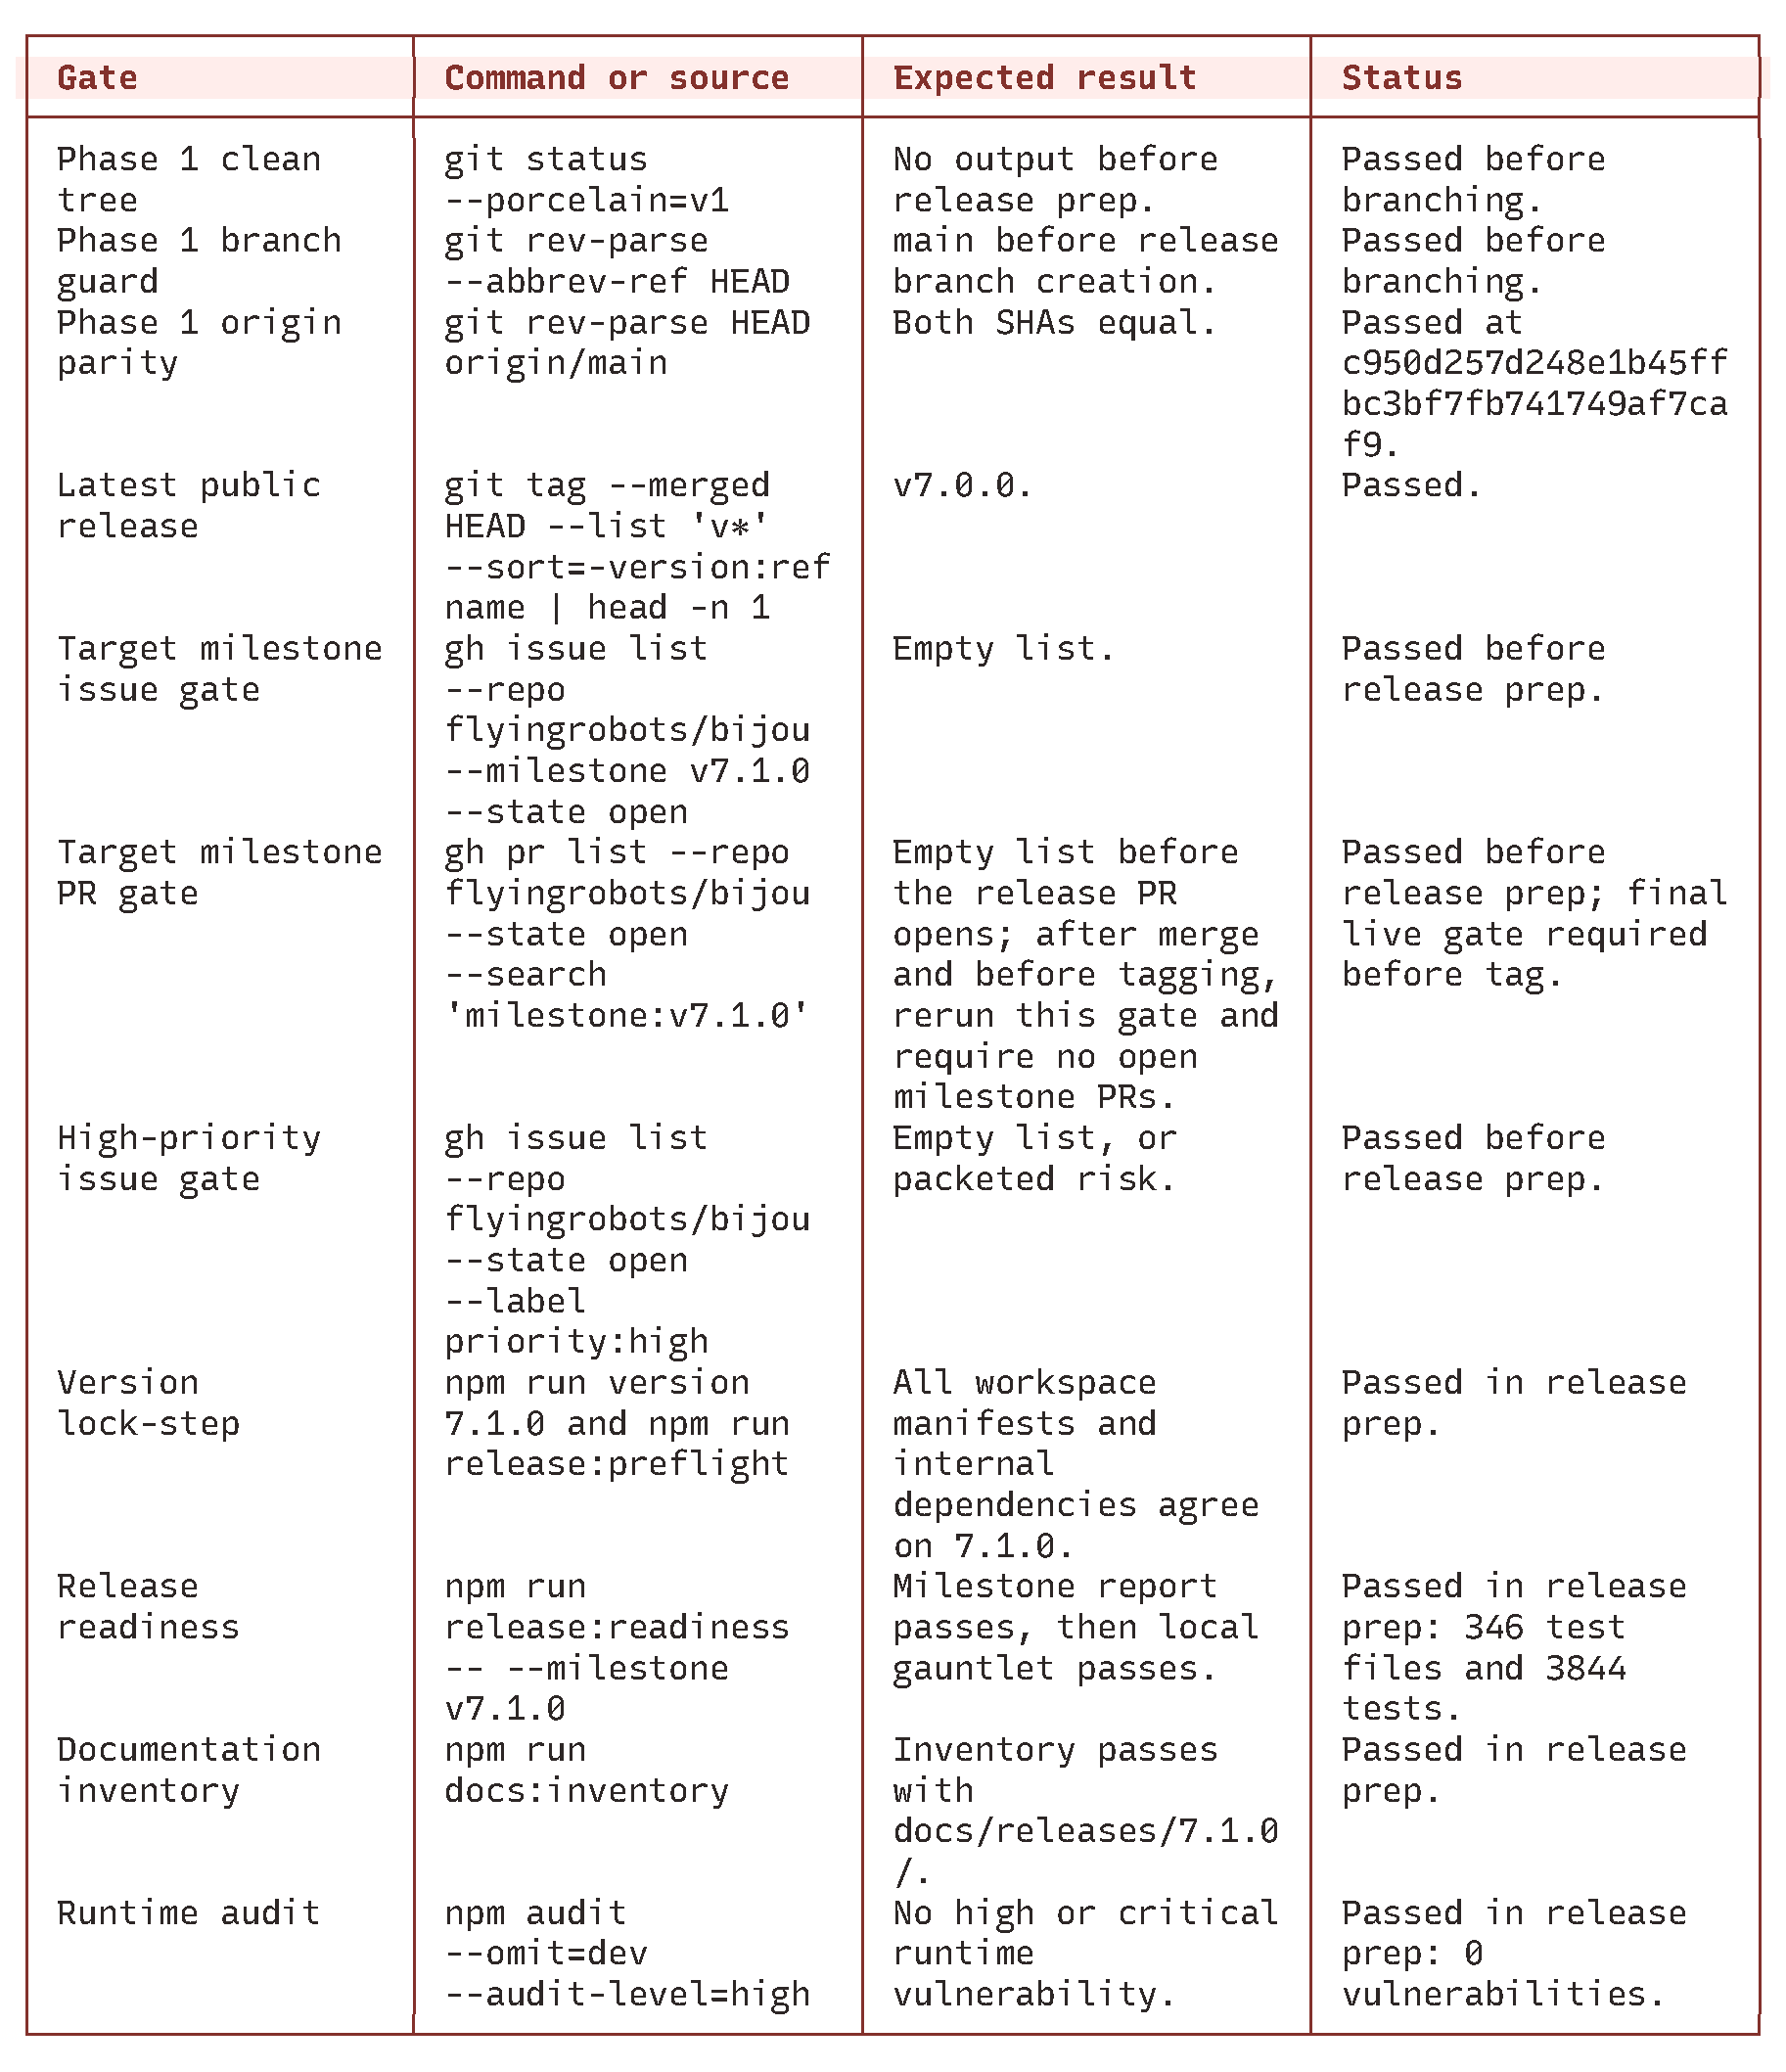
\includegraphics[width=\linewidth]{figures/tables/table-065-g1-1.pdf}
\par\smallskip{\scriptsize\color{BookMuted}Rows 1–11. Actual Bijou table component.}
\end{center}
\par\medskip
\begin{center}
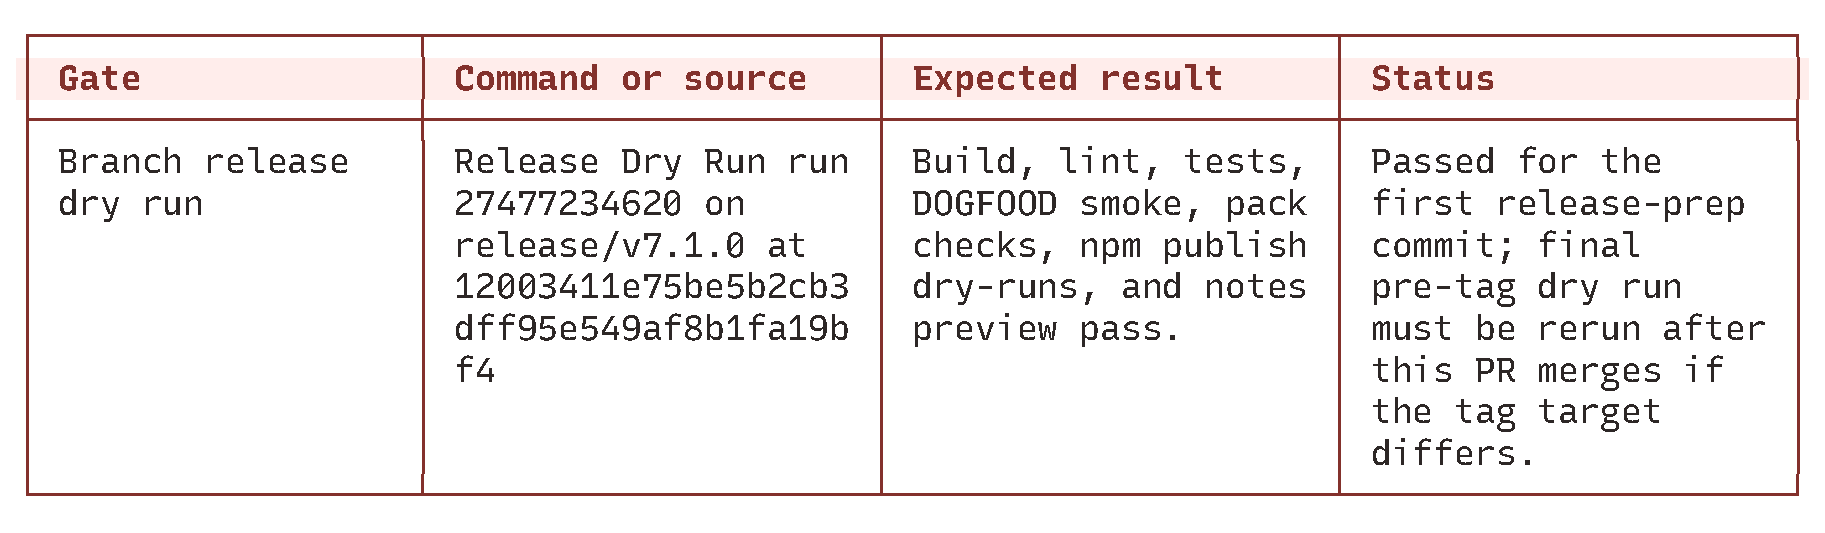
\includegraphics[width=\linewidth]{figures/tables/table-065-g1-2.pdf}
\par\smallskip{\scriptsize\color{BookMuted}Rows 12–12. Actual Bijou table component.}
\end{center}


\section{Human Review Matrix}\label{record-260-human-review-matrix}

\begin{center}
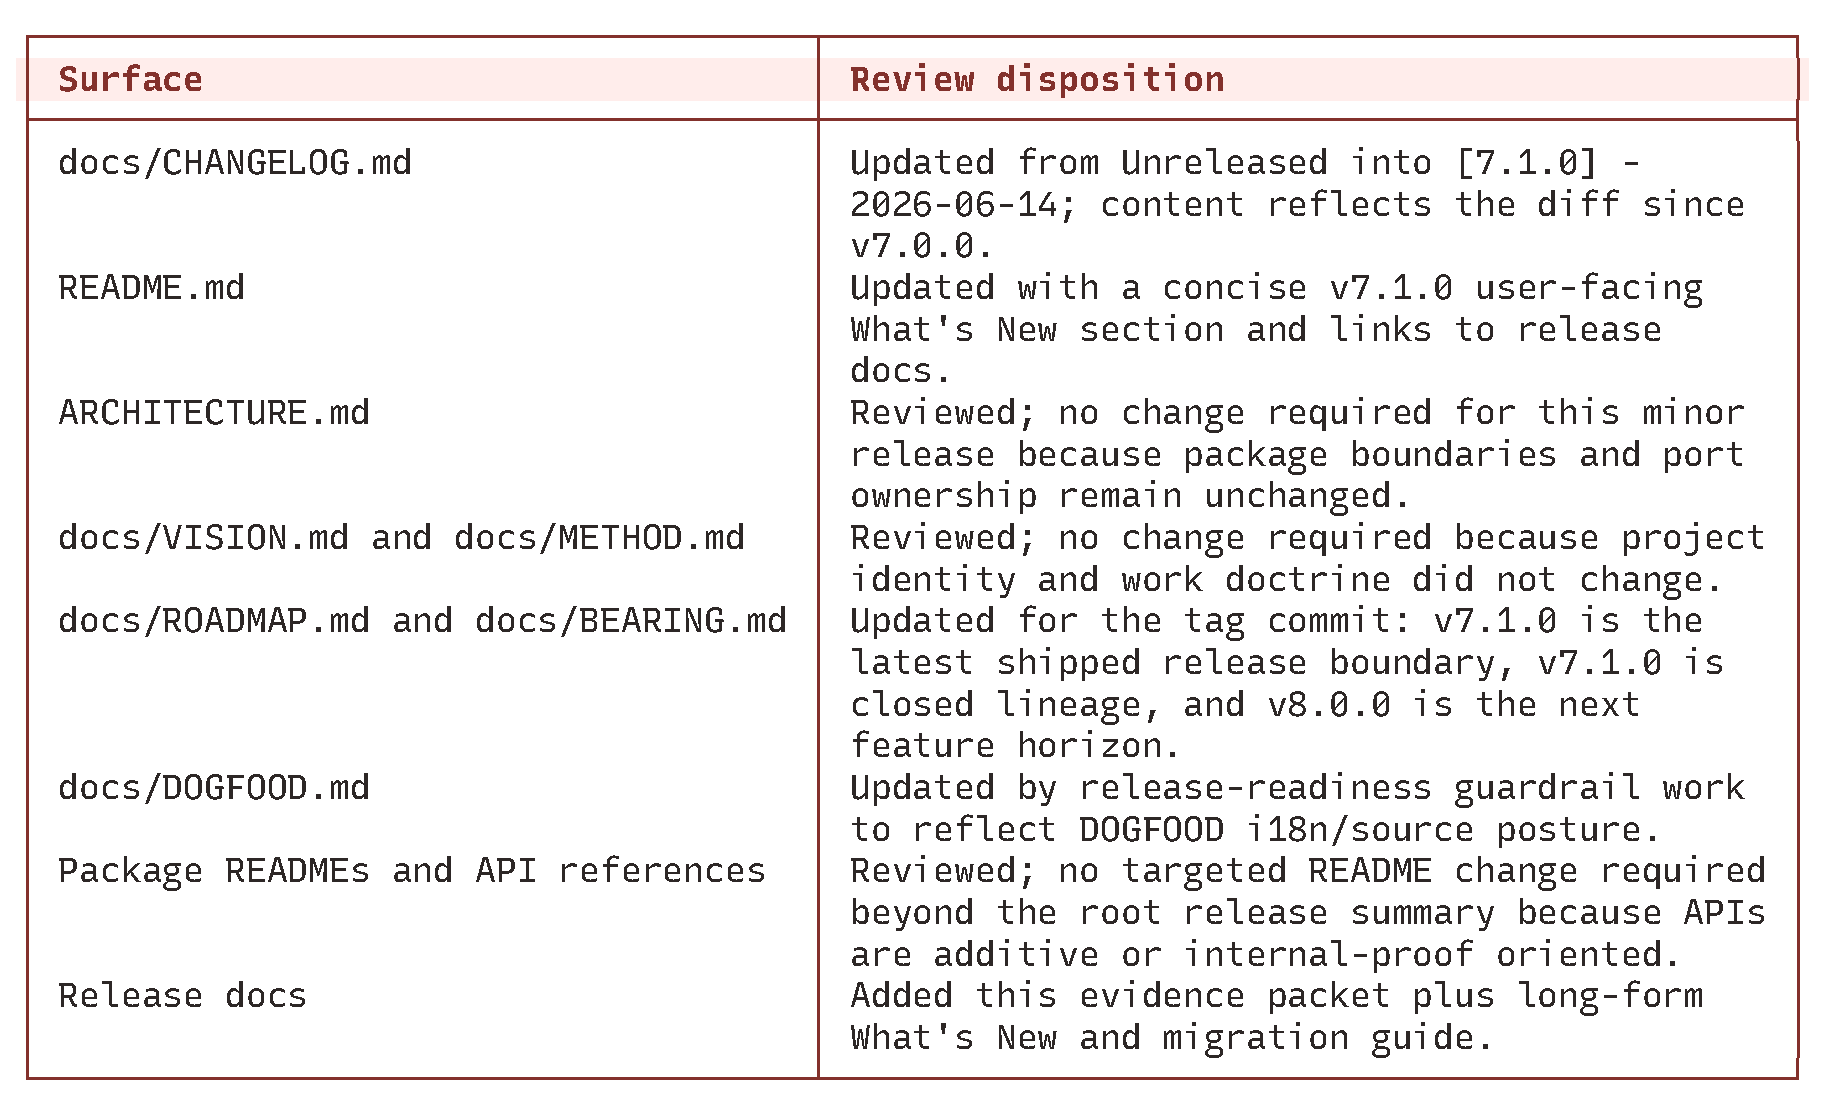
\includegraphics[width=\linewidth]{figures/tables/table-066-g1-1.pdf}
\par\smallskip{\scriptsize\color{BookMuted}Rows 1–8. Actual Bijou table component.}
\end{center}


\section{Deterministic Reproducibility Record}\label{record-260-deterministic-reproducibility-record}

\begin{center}
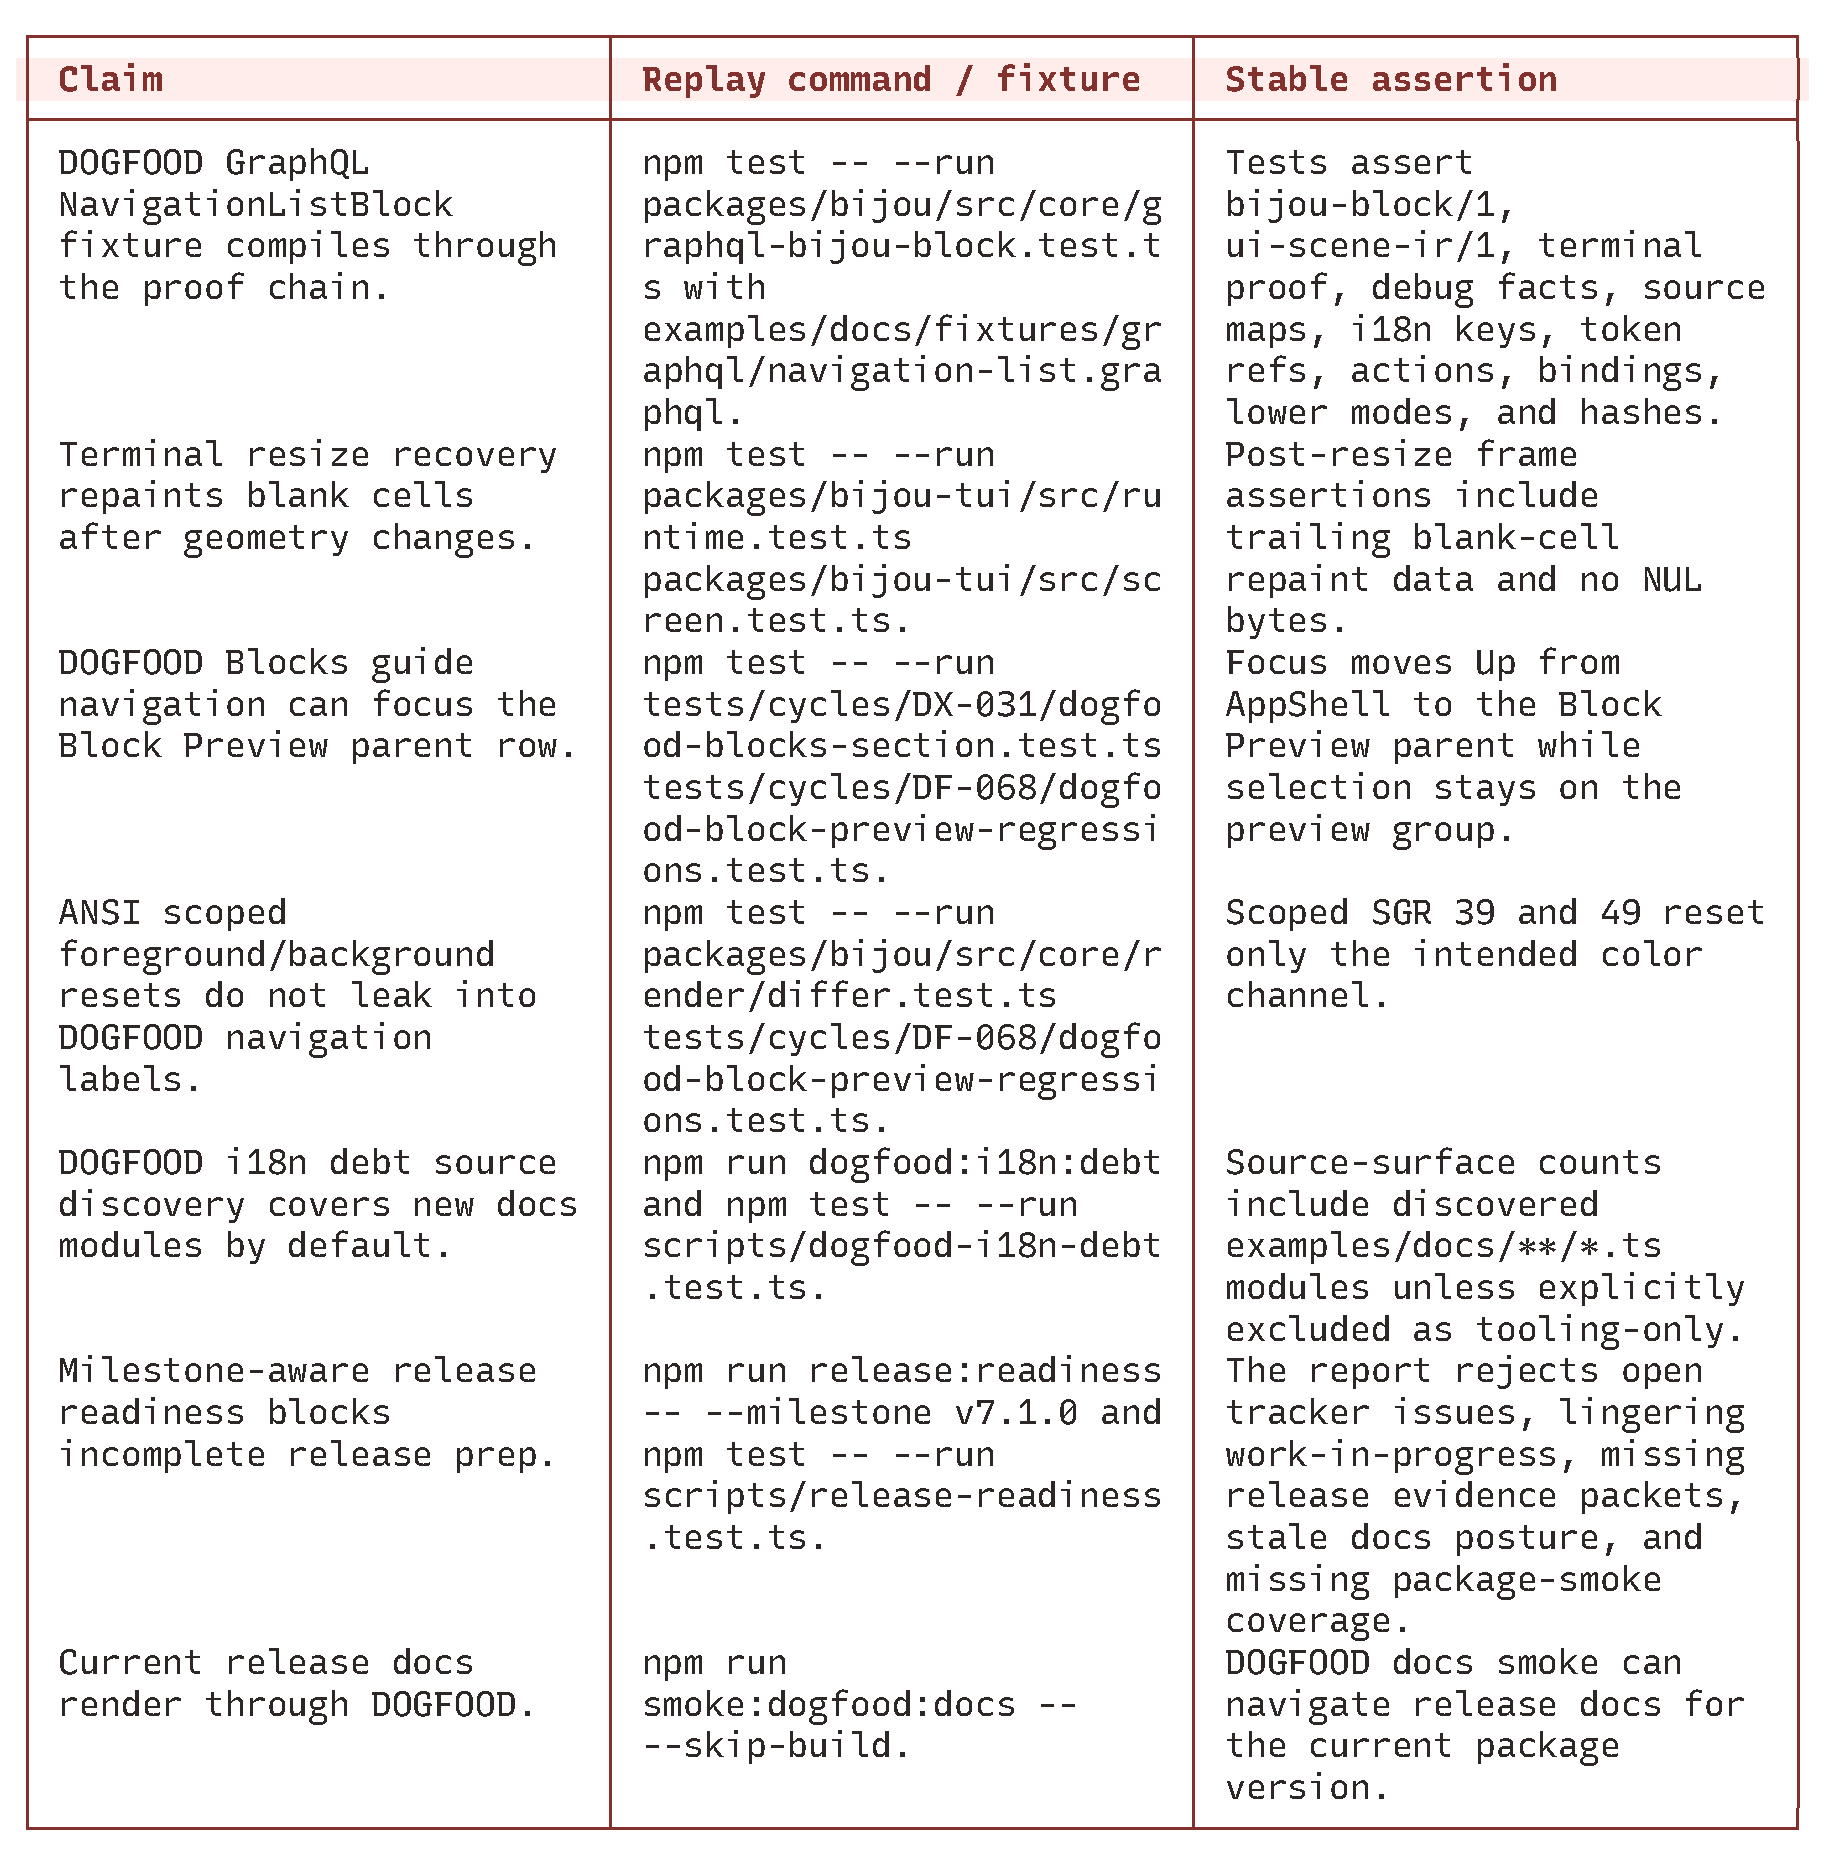
\includegraphics[width=\linewidth]{figures/tables/table-067-g1-1.pdf}
\par\smallskip{\scriptsize\color{BookMuted}Rows 1–7. Actual Bijou table component.}
\end{center}


\section{Package And Registry Verification Plan}\label{record-260-package-and-registry-verification-plan}

After the release PR is merged and only after explicit operator approval to tag:

\begin{enumerate}
\def\labelenumi{\arabic{enumi}.}
\tightlist
\item
  Fast-forward local \texttt{m\allowbreak{}a\allowbreak{}i\allowbreak{}n} to the exact \texttt{o\allowbreak{}r\allowbreak{}i\allowbreak{}g\allowbreak{}i\allowbreak{}n\allowbreak{}/\allowbreak{}m\allowbreak{}a\allowbreak{}i\allowbreak{}n} release commit.
\item
  Re-run the live tracker gates: \texttt{g\allowbreak{}h\allowbreak{} \allowbreak{}i\allowbreak{}s\allowbreak{}s\allowbreak{}u\allowbreak{}e\allowbreak{} \allowbreak{}l\allowbreak{}i\allowbreak{}s\allowbreak{}t\allowbreak{} \allowbreak{}-\allowbreak{}-\allowbreak{}r\allowbreak{}e\allowbreak{}p\allowbreak{}o\allowbreak{} \allowbreak{}f\allowbreak{}l\allowbreak{}y\allowbreak{}i\allowbreak{}n\allowbreak{}g\allowbreak{}r\allowbreak{}o\allowbreak{}b\allowbreak{}o\allowbreak{}t\allowbreak{}s\allowbreak{}/\allowbreak{}b\allowbreak{}i\allowbreak{}j\allowbreak{}o\allowbreak{}u\allowbreak{} \allowbreak{}-\allowbreak{}-\allowbreak{}m\allowbreak{}i\allowbreak{}l\allowbreak{}e\allowbreak{}s\allowbreak{}t\allowbreak{}o\allowbreak{}n\allowbreak{}e\allowbreak{} \allowbreak{}v\allowbreak{}7\allowbreak{}.\allowbreak{}1\allowbreak{}.\allowbreak{}0\allowbreak{} \allowbreak{}-\allowbreak{}-\allowbreak{}s\allowbreak{}t\allowbreak{}a\allowbreak{}t\allowbreak{}e\allowbreak{} \allowbreak{}o\allowbreak{}p\allowbreak{}e\allowbreak{}n}, \texttt{g\allowbreak{}h\allowbreak{} \allowbreak{}p\allowbreak{}r\allowbreak{} \allowbreak{}l\allowbreak{}i\allowbreak{}s\allowbreak{}t\allowbreak{} \allowbreak{}-\allowbreak{}-\allowbreak{}r\allowbreak{}e\allowbreak{}p\allowbreak{}o\allowbreak{} \allowbreak{}f\allowbreak{}l\allowbreak{}y\allowbreak{}i\allowbreak{}n\allowbreak{}g\allowbreak{}r\allowbreak{}o\allowbreak{}b\allowbreak{}o\allowbreak{}t\allowbreak{}s\allowbreak{}/\allowbreak{}b\allowbreak{}i\allowbreak{}j\allowbreak{}o\allowbreak{}u\allowbreak{} \allowbreak{}-\allowbreak{}-\allowbreak{}s\allowbreak{}t\allowbreak{}a\allowbreak{}t\allowbreak{}e\allowbreak{} \allowbreak{}o\allowbreak{}p\allowbreak{}e\allowbreak{}n\allowbreak{} \allowbreak{}-\allowbreak{}-\allowbreak{}s\allowbreak{}e\allowbreak{}a\allowbreak{}r\allowbreak{}c\allowbreak{}h\allowbreak{} \allowbreak{}'\allowbreak{}m\allowbreak{}i\allowbreak{}l\allowbreak{}e\allowbreak{}s\allowbreak{}t\allowbreak{}o\allowbreak{}n\allowbreak{}e\allowbreak{}:\allowbreak{}v\allowbreak{}7\allowbreak{}.\allowbreak{}1\allowbreak{}.\allowbreak{}0\allowbreak{}'}, and \texttt{g\allowbreak{}h\allowbreak{} \allowbreak{}i\allowbreak{}s\allowbreak{}s\allowbreak{}u\allowbreak{}e\allowbreak{} \allowbreak{}l\allowbreak{}i\allowbreak{}s\allowbreak{}t\allowbreak{} \allowbreak{}-\allowbreak{}-\allowbreak{}r\allowbreak{}e\allowbreak{}p\allowbreak{}o\allowbreak{} \allowbreak{}f\allowbreak{}l\allowbreak{}y\allowbreak{}i\allowbreak{}n\allowbreak{}g\allowbreak{}r\allowbreak{}o\allowbreak{}b\allowbreak{}o\allowbreak{}t\allowbreak{}s\allowbreak{}/\allowbreak{}b\allowbreak{}i\allowbreak{}j\allowbreak{}o\allowbreak{}u\allowbreak{} \allowbreak{}-\allowbreak{}-\allowbreak{}s\allowbreak{}t\allowbreak{}a\allowbreak{}t\allowbreak{}e\allowbreak{} \allowbreak{}o\allowbreak{}p\allowbreak{}e\allowbreak{}n\allowbreak{} \allowbreak{}-\allowbreak{}-\allowbreak{}l\allowbreak{}a\allowbreak{}b\allowbreak{}e\allowbreak{}l\allowbreak{} \allowbreak{}p\allowbreak{}r\allowbreak{}i\allowbreak{}o\allowbreak{}r\allowbreak{}i\allowbreak{}t\allowbreak{}y\allowbreak{}:\allowbreak{}h\allowbreak{}i\allowbreak{}g\allowbreak{}h}. Abort before tagging if any release-blocking item appears without an explicit packeted risk disposition.
\item
  Re-run \texttt{n\allowbreak{}p\allowbreak{}m\allowbreak{} \allowbreak{}r\allowbreak{}u\allowbreak{}n\allowbreak{} \allowbreak{}r\allowbreak{}e\allowbreak{}l\allowbreak{}e\allowbreak{}a\allowbreak{}s\allowbreak{}e\allowbreak{}:\allowbreak{}p\allowbreak{}r\allowbreak{}e\allowbreak{}f\allowbreak{}l\allowbreak{}i\allowbreak{}g\allowbreak{}h\allowbreak{}t} and \texttt{n\allowbreak{}p\allowbreak{}m\allowbreak{} \allowbreak{}r\allowbreak{}u\allowbreak{}n\allowbreak{} \allowbreak{}d\allowbreak{}o\allowbreak{}c\allowbreak{}s\allowbreak{}:\allowbreak{}i\allowbreak{}n\allowbreak{}v\allowbreak{}e\allowbreak{}n\allowbreak{}t\allowbreak{}o\allowbreak{}r\allowbreak{}y}.
\item
  Run the Release Dry Run workflow against the exact merged release commit, or against the release branch head only if it still matches the tag target. Record the run URL and abort before tagging if the run is not green.
\item
  Create the annotated \texttt{v\allowbreak{}7\allowbreak{}.\allowbreak{}1\allowbreak{}.\allowbreak{}0} tag from clean synced \texttt{m\allowbreak{}a\allowbreak{}i\allowbreak{}n}.
\item
  Push only \texttt{v\allowbreak{}7\allowbreak{}.\allowbreak{}1\allowbreak{}.\allowbreak{}0}.
\item
  Verify tag guard and publish workflows pass.
\item
  Verify npm reports \texttt{7\allowbreak{}.\allowbreak{}1\allowbreak{}.\allowbreak{}0} and \texttt{l\allowbreak{}a\allowbreak{}t\allowbreak{}e\allowbreak{}s\allowbreak{}t} for each automated publish package: \texttt{@\allowbreak{}f\allowbreak{}l\allowbreak{}y\allowbreak{}i\allowbreak{}n\allowbreak{}g\allowbreak{}r\allowbreak{}o\allowbreak{}b\allowbreak{}o\allowbreak{}t\allowbreak{}s\allowbreak{}/\allowbreak{}b\allowbreak{}i\allowbreak{}j\allowbreak{}o\allowbreak{}u}, \texttt{@\allowbreak{}f\allowbreak{}l\allowbreak{}y\allowbreak{}i\allowbreak{}n\allowbreak{}g\allowbreak{}r\allowbreak{}o\allowbreak{}b\allowbreak{}o\allowbreak{}t\allowbreak{}s\allowbreak{}/\allowbreak{}b\allowbreak{}i\allowbreak{}j\allowbreak{}o\allowbreak{}u\allowbreak{}-\allowbreak{}n\allowbreak{}o\allowbreak{}d\allowbreak{}e}, \texttt{@\allowbreak{}f\allowbreak{}l\allowbreak{}y\allowbreak{}i\allowbreak{}n\allowbreak{}g\allowbreak{}r\allowbreak{}o\allowbreak{}b\allowbreak{}o\allowbreak{}t\allowbreak{}s\allowbreak{}/\allowbreak{}b\allowbreak{}i\allowbreak{}j\allowbreak{}o\allowbreak{}u\allowbreak{}-\allowbreak{}t\allowbreak{}u\allowbreak{}i}, \texttt{@\allowbreak{}f\allowbreak{}l\allowbreak{}y\allowbreak{}i\allowbreak{}n\allowbreak{}g\allowbreak{}r\allowbreak{}o\allowbreak{}b\allowbreak{}o\allowbreak{}t\allowbreak{}s\allowbreak{}/\allowbreak{}b\allowbreak{}i\allowbreak{}j\allowbreak{}o\allowbreak{}u\allowbreak{}-\allowbreak{}t\allowbreak{}u\allowbreak{}i\allowbreak{}-\allowbreak{}a\allowbreak{}p\allowbreak{}p}, \texttt{c\allowbreak{}r\allowbreak{}e\allowbreak{}a\allowbreak{}t\allowbreak{}e\allowbreak{}-\allowbreak{}b\allowbreak{}i\allowbreak{}j\allowbreak{}o\allowbreak{}u\allowbreak{}-\allowbreak{}t\allowbreak{}u\allowbreak{}i\allowbreak{}-\allowbreak{}a\allowbreak{}p\allowbreak{}p}, \texttt{@\allowbreak{}f\allowbreak{}l\allowbreak{}y\allowbreak{}i\allowbreak{}n\allowbreak{}g\allowbreak{}r\allowbreak{}o\allowbreak{}b\allowbreak{}o\allowbreak{}t\allowbreak{}s\allowbreak{}/\allowbreak{}b\allowbreak{}i\allowbreak{}j\allowbreak{}o\allowbreak{}u\allowbreak{}-\allowbreak{}i\allowbreak{}1\allowbreak{}8\allowbreak{}n}, \texttt{@\allowbreak{}f\allowbreak{}l\allowbreak{}y\allowbreak{}i\allowbreak{}n\allowbreak{}g\allowbreak{}r\allowbreak{}o\allowbreak{}b\allowbreak{}o\allowbreak{}t\allowbreak{}s\allowbreak{}/\allowbreak{}b\allowbreak{}i\allowbreak{}j\allowbreak{}o\allowbreak{}u\allowbreak{}-\allowbreak{}i\allowbreak{}1\allowbreak{}8\allowbreak{}n\allowbreak{}-\allowbreak{}t\allowbreak{}o\allowbreak{}o\allowbreak{}l\allowbreak{}s}, \texttt{@\allowbreak{}f\allowbreak{}l\allowbreak{}y\allowbreak{}i\allowbreak{}n\allowbreak{}g\allowbreak{}r\allowbreak{}o\allowbreak{}b\allowbreak{}o\allowbreak{}t\allowbreak{}s\allowbreak{}/\allowbreak{}b\allowbreak{}i\allowbreak{}j\allowbreak{}o\allowbreak{}u\allowbreak{}-\allowbreak{}i\allowbreak{}1\allowbreak{}8\allowbreak{}n\allowbreak{}-\allowbreak{}t\allowbreak{}o\allowbreak{}o\allowbreak{}l\allowbreak{}s\allowbreak{}-\allowbreak{}n\allowbreak{}o\allowbreak{}d\allowbreak{}e}, \texttt{@\allowbreak{}f\allowbreak{}l\allowbreak{}y\allowbreak{}i\allowbreak{}n\allowbreak{}g\allowbreak{}r\allowbreak{}o\allowbreak{}b\allowbreak{}o\allowbreak{}t\allowbreak{}s\allowbreak{}/\allowbreak{}b\allowbreak{}i\allowbreak{}j\allowbreak{}o\allowbreak{}u\allowbreak{}-\allowbreak{}i\allowbreak{}1\allowbreak{}8\allowbreak{}n\allowbreak{}-\allowbreak{}t\allowbreak{}o\allowbreak{}o\allowbreak{}l\allowbreak{}s\allowbreak{}-\allowbreak{}x\allowbreak{}l\allowbreak{}s\allowbreak{}x}, and \texttt{@\allowbreak{}f\allowbreak{}l\allowbreak{}y\allowbreak{}i\allowbreak{}n\allowbreak{}g\allowbreak{}r\allowbreak{}o\allowbreak{}b\allowbreak{}o\allowbreak{}t\allowbreak{}s\allowbreak{}/\allowbreak{}b\allowbreak{}i\allowbreak{}j\allowbreak{}o\allowbreak{}u\allowbreak{}-\allowbreak{}m\allowbreak{}c\allowbreak{}p}.
\item
  Verify the GitHub Release exists with generated notes.
\end{enumerate}

\section{Residual Risk}\label{record-260-residual-risk}

\begin{itemize}
\tightlist
\item
  A branch dry-run workflow passed for an earlier release-prep commit. Because this packet changed after that run, the final pre-tag Release Dry Run must be rerun on the exact merged release commit before tag creation. The final tag guard, publish workflow, npm registry verification, and GitHub Release verification still cannot occur in this prep pass because the operator explicitly prohibited tag creation and tag pushes.
\item
  The broad Runtime Graph and Scene IR product contract remains V8 work. The 7.1.0 release intentionally ships proof slices and guardrails only.
\end{itemize}

No accepted unresolved high-priority issue is recorded for this release packet.

